\documentclass[twoside]{book}

% Packages required by doxygen
\usepackage{fixltx2e}
\usepackage{calc}
\usepackage{doxygen}
\usepackage[export]{adjustbox} % also loads graphicx
\usepackage{graphicx}
\usepackage[utf8]{inputenc}
\usepackage{makeidx}
\usepackage{multicol}
\usepackage{multirow}
\PassOptionsToPackage{warn}{textcomp}
\usepackage{textcomp}
\usepackage[nointegrals]{wasysym}
\usepackage[table]{xcolor}

% Font selection
\usepackage[T1]{fontenc}
\usepackage[scaled=.90]{helvet}
\usepackage{courier}
\usepackage{amssymb}
\usepackage{sectsty}
\renewcommand{\familydefault}{\sfdefault}
\allsectionsfont{%
  \fontseries{bc}\selectfont%
  \color{darkgray}%
}
\renewcommand{\DoxyLabelFont}{%
  \fontseries{bc}\selectfont%
  \color{darkgray}%
}
\newcommand{\+}{\discretionary{\mbox{\scriptsize$\hookleftarrow$}}{}{}}

% Page & text layout
\usepackage{geometry}
\geometry{%
  a4paper,%
  top=2.5cm,%
  bottom=2.5cm,%
  left=2.5cm,%
  right=2.5cm%
}
\tolerance=750
\hfuzz=15pt
\hbadness=750
\setlength{\emergencystretch}{15pt}
\setlength{\parindent}{0cm}
\setlength{\parskip}{3ex plus 2ex minus 2ex}
\makeatletter
\renewcommand{\paragraph}{%
  \@startsection{paragraph}{4}{0ex}{-1.0ex}{1.0ex}{%
    \normalfont\normalsize\bfseries\SS@parafont%
  }%
}
\renewcommand{\subparagraph}{%
  \@startsection{subparagraph}{5}{0ex}{-1.0ex}{1.0ex}{%
    \normalfont\normalsize\bfseries\SS@subparafont%
  }%
}
\makeatother

% Headers & footers
\usepackage{fancyhdr}
\pagestyle{fancyplain}
\fancyhead[LE]{\fancyplain{}{\bfseries\thepage}}
\fancyhead[CE]{\fancyplain{}{}}
\fancyhead[RE]{\fancyplain{}{\bfseries\leftmark}}
\fancyhead[LO]{\fancyplain{}{\bfseries\rightmark}}
\fancyhead[CO]{\fancyplain{}{}}
\fancyhead[RO]{\fancyplain{}{\bfseries\thepage}}
\fancyfoot[LE]{\fancyplain{}{}}
\fancyfoot[CE]{\fancyplain{}{}}
\fancyfoot[RE]{\fancyplain{}{\bfseries\scriptsize Generated by Doxygen }}
\fancyfoot[LO]{\fancyplain{}{\bfseries\scriptsize Generated by Doxygen }}
\fancyfoot[CO]{\fancyplain{}{}}
\fancyfoot[RO]{\fancyplain{}{}}
\renewcommand{\footrulewidth}{0.4pt}
\renewcommand{\chaptermark}[1]{%
  \markboth{#1}{}%
}
\renewcommand{\sectionmark}[1]{%
  \markright{\thesection\ #1}%
}

% Indices & bibliography
\usepackage{natbib}
\usepackage[titles]{tocloft}
\setcounter{tocdepth}{3}
\setcounter{secnumdepth}{5}
\makeindex

% Hyperlinks (required, but should be loaded last)
\usepackage{ifpdf}
\ifpdf
  \usepackage[pdftex,pagebackref=true]{hyperref}
\else
  \usepackage[ps2pdf,pagebackref=true]{hyperref}
\fi
\hypersetup{%
  colorlinks=true,%
  linkcolor=blue,%
  citecolor=blue,%
  unicode%
}

% Custom commands
\newcommand{\clearemptydoublepage}{%
  \newpage{\pagestyle{empty}\cleardoublepage}%
}

\usepackage{caption}
\captionsetup{labelsep=space,justification=centering,font={bf},singlelinecheck=off,skip=4pt,position=top}

%===== C O N T E N T S =====

\begin{document}

% Titlepage & ToC
\hypersetup{pageanchor=false,
             bookmarksnumbered=true,
             pdfencoding=unicode
            }
\pagenumbering{alph}
\begin{titlepage}
\vspace*{7cm}
\begin{center}%
{\Large Reconstruction }\\
\vspace*{1cm}
{\large Generated by Doxygen 1.8.13}\\
\end{center}
\end{titlepage}
\clearemptydoublepage
\pagenumbering{roman}
\tableofcontents
\clearemptydoublepage
\pagenumbering{arabic}
\hypersetup{pageanchor=true}

%--- Begin generated contents ---
\chapter{Reconstruction\+:}
\label{index}\hypertarget{index}{}Threading,Synchronisation and Data Integrity. An aircraft is patrolling space surrounding a base station. The aircrafts task is to localise enemy aircraft (bogies) that enters the airspace and intercept the aircraft.\hypertarget{index_Description}{}\section{Description}\label{index_Description}
Write a program in C++ using object oriented paradigms that shares data originating from a range of Mechatronics sensors between a number of threads. Ensure data integrity between threads and enable relating data between them via suitable data structure that enables time synchronisation and subsequently interpolation of data for task at hand. Supply appropriate auto-\/generated documentation utilising inline source mark-\/up\hypertarget{index_Rationale}{}\subsection{Rationale}\label{index_Rationale}
In a Mechatronics System, sensors produce data at varying rates. Decisions need to be made based on correctly associated data in near real-\/time. Threading and synchronisation are ways to ensure the system performs as intended, with guarantees on the responsiveness of the system to incoming data changes, processing constraints and system behaviour.\hypertarget{index_Details}{}\section{Details}\label{index_Details}

\begin{DoxyItemize}
\item Student Name\+: Esteban Andrade~\newline

\item Student ID\+: 12824583
\end{DoxyItemize}\hypertarget{index_Notes}{}\section{Notes}\label{index_Notes}
There is a debug section in the Data\+Synchronization Class. This was used for debugging all the predictions based on the speed and locations of the bogies.

\begin{DoxyVerb}//#define DEBUG 1
Uncomment this section to allow this to be displayed.\end{DoxyVerb}
\hypertarget{index_Algorithms}{}\section{Algorithms}\label{index_Algorithms}
The algorithms and concepts used include\+:
\begin{DoxyItemize}
\item Pure Pursuit
\item P Cotroller
\item Projectile Motion
\end{DoxyItemize}\hypertarget{index_ac_doc_}{}\subsection{Pure Pursuit}\label{index_ac_doc_}
The Pure pursuit Algorith will be used in order to start chansing the bogies The heart of the pure pursuit controller is directing the aircraft to travel along an arc from the current location to the goal point. This goal point is called the ​ lookahead point ​ and it is a point on the path that is the ​ lookahead distance from the aircraft. As the robot moves along the path, it aims for the lookahead point, which moves down the path with the robot. In this way, the robot can be considered to “pursue” the lookahead point. The lookahead point will be the predicted bogie position All this analysis will be done in reference from the friendly to the bogie. The point ( x, y ) which is one look-\/ahead distance l from the robot is one of points on the path.\+The Formulas include \begin{DoxyVerb}  x^2 +y^2 = L^2
  x+D = r
  D = r-x
  (r-x)^2+y^2=r^2
  r^2-2rx+x^2+y^2=r^2
  2rx=L^2
  r= L^2/2x
  gamma = 2x/L^2

  In order to obtain x, using ax+by+c=0
 a = − tan(robot angle)
 b =1
 c = tan(robot angle) * robot x − robot y
 The point-line distance formula is:
 d = | ax + b y + c | / √ {a^2 + b^2}
 x = | a * lookahead x + b * lookahead y + c | / √{a^2 + b^2}
 with this angle gamma we can have a relationship between the linear and angular velocity:
 w(omega) = gamma *(linear velocity)
\end{DoxyVerb}
\hypertarget{index_ac_doc_PI_Cotroller}{}\subsection{P\+I Cotroller}\label{index_ac_doc_PI_Cotroller}
A PI controller was used in order to improve the navigation and steering paramaters. Where a gain K will be used to make the friendly either\+:
\begin{DoxyItemize}
\item Turn fast toward look-\/ahead point direction.
\item Turn slowly toward look-\/ahead point direction
\end{DoxyItemize}

This gain will either increase or decrease both angular speed and linear speed in order to improve navigation. \begin{DoxyVerb}This value was simplifies as K, in order to maintain the 6G constrain and be easily modified 
Kp+KI/s
K+K/s
\end{DoxyVerb}
\hypertarget{index_ac_doc_Projectile_Motion}{}\subsection{Projectile Motion}\label{index_ac_doc_Projectile_Motion}
The concept of projectile motion was used in order to predict the future position of the bogies. For this two simple positions with their respective timestamp were taken. With this we can calculate the distance travelled in x and y and with the given different in timestamp we can obtain the velocity vector. Once the velocity vector was used and gith a given offset in time in the future we can predict the future location of the bogies. \begin{DoxyVerb}vx = (second x - original x) /  time difference
vy = (second y - original y) /  time difference
predicted x = second x + velocity x * (time difference + future offset);
predicted y = second y + velocity y * (time difference + future offset);
\end{DoxyVerb}
\hypertarget{index_Notes}{}\subsection{Notes}\label{index_Notes}
In occasions the predicted orientation will have a small offset. However it will adjust and correct itself after a few iterations 
\chapter{3\+D-\/\+Reconstructrion-\/\+Scanner}
\label{md_README}
\Hypertarget{md_README}
{\bfseries Author\+: Esteban Andrade}

This will be the developed framework software for a 3D software. This framework will use phogrammetric software to produce the reconstruction and a series of algorithms that are used in this framework.

The framework will be used for processing, filtering, scaling and reconstructing the final mesh obtained from the photogrammetric process.

\subsection*{Meshroom}

Meshroom is the photogrammetric software used for 3D reconstruction. In this software a series of images will be loaded and it will reconstruct the required Scenes. It is compatible with Linux and Windows.

Both platforms worked for this project of the 3D scanner. Both Version 2020 and 2021 were used and the results were consistent between each other using the same settings.

\subsubsection*{Requirements}

N\+V\+I\+D\+IA C\+U\+D\+A-\/enabled G\+PU (built with cuda-\/10 compatible with compute capability 3.\+0 to 7.\+5)

\paragraph*{Installation}

Meshroom can be installed with the following links.


\begin{DoxyItemize}
\item \href{https://github.com/alicevision/meshroom}{\tt Git\+Hub Repo}.
\item \href{https://alicevision.org/#meshroom}{\tt Alice Vision}
\end{DoxyItemize}

\subsubsection*{How to use}

The respective settings and best configuration for each node can be referenced on the Thesis document \href{https://github.com/esteban-andrade/3D-Reconstructrion-Scanner/blob/main/A21%20-%2004017%20Final%20Report%20Esteban%20Andrade%20Zambrano.pdf}{\tt Documentation}.

In the above documents there will be documentation of what settings are required for each node. (Refer to section 2.\+2 on the \href{https://github.com/esteban-andrade/3D-Reconstructrion-Scanner/blob/main/A21%20-%2004017%20Final%20Report%20Esteban%20Andrade%20Zambrano.pdf}{\tt Documentation}).

Once the photogrammetric process has finished the mesh can be retrieved from either the {\itshape meshing} or {\itshape filter mesh node} as ..obj file from the cache folder from meshroom.

For best result, as these meshes will be used in the {\itshape \hyperlink{classReconstruction}{Reconstruction} Framework}, convert the meshes from $\ast$.obj$\ast$ to $\ast$.ply$\ast$ using {\bfseries \href{https://www.meshlab.net/}{\tt Meshlab}}.

\subsection*{\hyperlink{classReconstruction}{Reconstruction} Framework.}

The reconstruction Framework is a series of classes and program that was develop in order to process, scale and recosstruct the Mesh result from Meshroom.

\subsubsection*{Requirements}

This framework was developed in Linux. However windows Functionality was added in order to build and compile the files.

The requirements include


\begin{DoxyItemize}
\item P\+CL Library $<$ 1.\+2
\item Open3D
\item Matlab
\item Open\+CV $<$= 3.\+9.\+2
\item Boost
\item C++ (14 Miniumum)
\item Python (3.\+6.\+9 Minimum)
\item Ninja Compiler (Optional).
\end{DoxyItemize}

\subsubsection*{Installation}

In order to install this framework its neccesary to build and compile this project.

\subparagraph*{Standard Method}


\begin{DoxyCode}
git clone https://github.com/esteban-andrade/3D-Reconstructrion-Scanner
mkdir build
cd build
cmake ..
make
\end{DoxyCode}
 \subparagraph*{Prefered Method}

The prefered method is using Ninja Compiler as it faster than standard gcc


\begin{DoxyCode}
git clone https://github.com/esteban-andrade/3D-Reconstructrion-Scanner
mkdir build
cd build
cmake -GNinja ..
ninja
\end{DoxyCode}


\subsubsection*{Execution}

In order to execute the framework it is neccesary to have two files $\ast$(.ply files)$\ast$ The first file has to be the target file that needs to be processed $\ast$(Output from meshrroom$\ast$. The second file has to be the file that will be used for scaling$\ast$(Lidar)$\ast$

The first term is the path to the reference target file. The second term is the path to the scale reference file. The last term is a command to generate output files. (Recommended to set to yes). All the output saved on the {\itshape Meshes Folder}

\#\#\#\#\# In order to execute\+: 
\begin{DoxyCode}
cd build 
/3D\_reconstruction\_pipeline [Path\_to\_referenceFile] [Path\_to\_SCaling\_file] [yes/no](Generate output files)
\end{DoxyCode}


\#\#\#\#\# Example 
\begin{DoxyCode}
./3D\_reconstruction\_pipeline ../Data/mesh\_ply.ply ../Data/10.ply no
\end{DoxyCode}


\paragraph*{Expected Result}

The expeted result will output a viewer with all the steps of the pipeline processing. If There is the need to change parameters, change then at the top of the {\itshape Reconstruction.\+cpp} file. To change the filtering adjust as needed on {\itshape main.\+cpp}. Ideally the default settings will work with most datasets.

\subparagraph*{Poisson \hyperlink{classReconstruction}{Reconstruction} Output.}

In certain occasions when the poisson reconstruction steps fails due to wrong normals direction. Possion script \href{https://github.com/esteban-andrade/3D-Reconstructrion-Scanner/blob/main/poisson_open3d.py}{\tt Possion Open3D}

This Script will require to use the output files from the process. (Ensure executable ({\itshape 3\+D\+\_\+reconstruction\+\_\+pipeline}) was set to {\bfseries Y\+ES}) This script will adjust the normals direction and run Poisson again.

To execute\+:


\begin{DoxyCode}
python3 poisson\_open3d.py
\end{DoxyCode}


\subsubsection*{Extra components}

An Extra component added and adapted to this framework is \href{https://github.com/linbaowei/ScaleRatioICP}{\tt S\+Cale\+Ratio\+I\+CP} The matlab components of this class were added here under \href{https://github.com/esteban-andrade/3D-Reconstructrion-Scanner}{\tt Scale\+Ratio\+I\+CP} In order to use this object ensure that {\bfseries Scale\+Ratio\+I\+C\+P.\+m} is added to the matlab path.

All the framework implementation was fully integrated and adapted. 
\chapter{Class Index}
\section{Class List}
Here are the classes, structs, unions and interfaces with brief descriptions\+:\begin{DoxyCompactList}
\item\contentsline{section}{\hyperlink{classaPoint}{a\+Point} \\*Class to handle points }{\pageref{classaPoint}}{}
\item\contentsline{section}{\hyperlink{classicp}{icp} \\*Main I\+CP class }{\pageref{classicp}}{}
\item\contentsline{section}{\hyperlink{classPoints3D}{Points3D} \\*Class to handle 3D points }{\pageref{classPoints3D}}{}
\item\contentsline{section}{\hyperlink{classPoints3Dvec}{Points3\+Dvec} \\*Class to handle Point vectors }{\pageref{classPoints3Dvec}}{}
\item\contentsline{section}{\hyperlink{classReconstruction}{Reconstruction} \\*The Class \hyperlink{classReconstruction}{Reconstruction} is used process the target pointcloud. It contain many implemeted algorithms used for filtering, segmentation, clusteting, etc }{\pageref{classReconstruction}}{}
\item\contentsline{section}{\hyperlink{structt__ply__}{t\+\_\+ply\+\_\+} }{\pageref{structt__ply__}}{}
\item\contentsline{section}{\hyperlink{structt__ply__argument__}{t\+\_\+ply\+\_\+argument\+\_\+} }{\pageref{structt__ply__argument__}}{}
\item\contentsline{section}{\hyperlink{structt__ply__element__}{t\+\_\+ply\+\_\+element\+\_\+} }{\pageref{structt__ply__element__}}{}
\item\contentsline{section}{\hyperlink{structt__ply__idriver__}{t\+\_\+ply\+\_\+idriver\+\_\+} }{\pageref{structt__ply__idriver__}}{}
\item\contentsline{section}{\hyperlink{structt__ply__odriver__}{t\+\_\+ply\+\_\+odriver\+\_\+} }{\pageref{structt__ply__odriver__}}{}
\item\contentsline{section}{\hyperlink{structt__ply__property__}{t\+\_\+ply\+\_\+property\+\_\+} }{\pageref{structt__ply__property__}}{}
\end{DoxyCompactList}

\chapter{File Index}
\section{File List}
Here is a list of all documented files with brief descriptions\+:\begin{DoxyCompactList}
\item\contentsline{section}{{\bfseries icp.\+h} }{\pageref{icp_8h}}{}
\item\contentsline{section}{\hyperlink{Reconstruction_8h}{Reconstruction.\+h} \\*This is the main class be used to hold all the A\+PI used for data processing }{\pageref{Reconstruction_8h}}{}
\item\contentsline{section}{{\bfseries rply.\+h} }{\pageref{rply_8h}}{}
\end{DoxyCompactList}

\chapter{Class Documentation}
\hypertarget{classaPoint}{}\section{a\+Point Class Reference}
\label{classaPoint}\index{a\+Point@{a\+Point}}


Class to handle points.  




{\ttfamily \#include $<$icp.\+h$>$}

\subsection*{Public Attributes}
\begin{DoxyCompactItemize}
\item 
\mbox{\Hypertarget{classaPoint_af1ef5dd62d225d264aceeb0728ac0ba7}\label{classaPoint_af1ef5dd62d225d264aceeb0728ac0ba7}} 
double {\bfseries x}
\item 
\mbox{\Hypertarget{classaPoint_aa8c73634208dd93e5572ca15e546ad39}\label{classaPoint_aa8c73634208dd93e5572ca15e546ad39}} 
double {\bfseries y}
\item 
\mbox{\Hypertarget{classaPoint_a0e221ad7ffa17d0c1dedd3073194cdc0}\label{classaPoint_a0e221ad7ffa17d0c1dedd3073194cdc0}} 
double {\bfseries z}
\end{DoxyCompactItemize}


\subsection{Detailed Description}
Class to handle points. 

The documentation for this class was generated from the following file\+:\begin{DoxyCompactItemize}
\item 
\hyperlink{icp_8h}{icp.\+h}\end{DoxyCompactItemize}

\hypertarget{classicp}{}\section{icp Class Reference}
\label{classicp}\index{icp@{icp}}


Main I\+CP class.  




{\ttfamily \#include $<$icp.\+h$>$}

\subsection*{Public Member Functions}
\begin{DoxyCompactItemize}
\item 
\hyperlink{classicp_a16dfbc3ddb18a613cfd4fb8861d0c16a}{icp} (std\+::string, int bin)
\begin{DoxyCompactList}\small\item\em Construct a new icp object. \end{DoxyCompactList}\item 
\mbox{\Hypertarget{classicp_a4f30b3d50f65a223095db3115d6393f2}\label{classicp_a4f30b3d50f65a223095db3115d6393f2}} 
\hyperlink{classicp_a4f30b3d50f65a223095db3115d6393f2}{icp} ()
\begin{DoxyCompactList}\small\item\em Construct a new icp object. \end{DoxyCompactList}\item 
\mbox{\Hypertarget{classicp_a4ddd15fc41c8005f7eaed9fb5b7ecf00}\label{classicp_a4ddd15fc41c8005f7eaed9fb5b7ecf00}} 
\hyperlink{classicp_a4ddd15fc41c8005f7eaed9fb5b7ecf00}{$\sim$icp} ()
\begin{DoxyCompactList}\small\item\em Destroy the icp object. \end{DoxyCompactList}\item 
void \hyperlink{classicp_aca508e79450dce34131b83ed2a4a1d95}{process\+Generation} (std\+::string, int bin)
\begin{DoxyCompactList}\small\item\em Start Process generation files. \end{DoxyCompactList}\item 
double \hyperlink{classicp_af5adbefb80bcd764306af7361e2a532a}{get\+I\+C\+Pscale} (std\+::vector$<$ std\+::string $>$ \&)
\begin{DoxyCompactList}\small\item\em Obtain the I\+CP scale. \end{DoxyCompactList}\end{DoxyCompactItemize}


\subsection{Detailed Description}
Main I\+CP class. 

\subsection{Constructor \& Destructor Documentation}
\mbox{\Hypertarget{classicp_a16dfbc3ddb18a613cfd4fb8861d0c16a}\label{classicp_a16dfbc3ddb18a613cfd4fb8861d0c16a}} 
\index{icp@{icp}!icp@{icp}}
\index{icp@{icp}!icp@{icp}}
\subsubsection{\texorpdfstring{icp()}{icp()}}
{\footnotesize\ttfamily icp\+::icp (\begin{DoxyParamCaption}\item[{std\+::string}]{plyname,  }\item[{int}]{bin }\end{DoxyParamCaption})}



Construct a new icp object. 


\begin{DoxyParams}{Parameters}
{\em plyname} & name of plyfile \\
\hline
{\em bin} & Image \\
\hline
\end{DoxyParams}


\subsection{Member Function Documentation}
\mbox{\Hypertarget{classicp_af5adbefb80bcd764306af7361e2a532a}\label{classicp_af5adbefb80bcd764306af7361e2a532a}} 
\index{icp@{icp}!get\+I\+C\+Pscale@{get\+I\+C\+Pscale}}
\index{get\+I\+C\+Pscale@{get\+I\+C\+Pscale}!icp@{icp}}
\subsubsection{\texorpdfstring{get\+I\+C\+Pscale()}{getICPscale()}}
{\footnotesize\ttfamily double icp\+::get\+I\+C\+Pscale (\begin{DoxyParamCaption}\item[{std\+::vector$<$ std\+::string $>$ \&}]{files }\end{DoxyParamCaption})}



Obtain the I\+CP scale. 


\begin{DoxyParams}{Parameters}
{\em files-\/} & vector of files names of process\+Generation output \\
\hline
\end{DoxyParams}
\begin{DoxyReturn}{Returns}
double (scale) 
\end{DoxyReturn}
\mbox{\Hypertarget{classicp_aca508e79450dce34131b83ed2a4a1d95}\label{classicp_aca508e79450dce34131b83ed2a4a1d95}} 
\index{icp@{icp}!process\+Generation@{process\+Generation}}
\index{process\+Generation@{process\+Generation}!icp@{icp}}
\subsubsection{\texorpdfstring{process\+Generation()}{processGeneration()}}
{\footnotesize\ttfamily void icp\+::process\+Generation (\begin{DoxyParamCaption}\item[{std\+::string}]{plyname,  }\item[{int}]{bin }\end{DoxyParamCaption})}



Start Process generation files. 


\begin{DoxyParams}{Parameters}
{\em plyname} & name of plyfile \\
\hline
{\em bin} & Image \\
\hline
{\em bin} & \\
\hline
\end{DoxyParams}


The documentation for this class was generated from the following files\+:\begin{DoxyCompactItemize}
\item 
\hyperlink{icp_8h}{icp.\+h}\item 
icp.\+cpp\end{DoxyCompactItemize}

\hypertarget{classPoints3D}{}\section{Points3D Class Reference}
\label{classPoints3D}\index{Points3D@{Points3D}}


Collaboration diagram for Points3D\+:\nopagebreak
\begin{figure}[H]
\begin{center}
\leavevmode
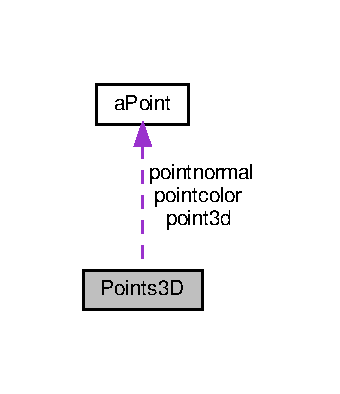
\includegraphics[width=163pt]{classPoints3D__coll__graph}
\end{center}
\end{figure}
\subsection*{Public Attributes}
\begin{DoxyCompactItemize}
\item 
\mbox{\Hypertarget{classPoints3D_ab83070a54a0f9857e76d20029c5c84f4}\label{classPoints3D_ab83070a54a0f9857e76d20029c5c84f4}} 
\hyperlink{classaPoint}{a\+Point} $\ast$ {\bfseries point3d}
\item 
\mbox{\Hypertarget{classPoints3D_af31fbf97956dcd4a50044942aa9b0d2f}\label{classPoints3D_af31fbf97956dcd4a50044942aa9b0d2f}} 
\hyperlink{classaPoint}{a\+Point} $\ast$ {\bfseries pointcolor}
\item 
\mbox{\Hypertarget{classPoints3D_ad24b7ace9209a787875a7ba5d7d299e6}\label{classPoints3D_ad24b7ace9209a787875a7ba5d7d299e6}} 
\hyperlink{classaPoint}{a\+Point} $\ast$ {\bfseries pointnormal}
\item 
\mbox{\Hypertarget{classPoints3D_a62b3884510bdabd40d1b6d70240a001f}\label{classPoints3D_a62b3884510bdabd40d1b6d70240a001f}} 
int {\bfseries point\+\_\+num}
\end{DoxyCompactItemize}


The documentation for this class was generated from the following file\+:\begin{DoxyCompactItemize}
\item 
icp.\+h\end{DoxyCompactItemize}

\hypertarget{classPoints3Dvec}{}\section{Points3\+Dvec Class Reference}
\label{classPoints3Dvec}\index{Points3\+Dvec@{Points3\+Dvec}}
\subsection*{Public Attributes}
\begin{DoxyCompactItemize}
\item 
\mbox{\Hypertarget{classPoints3Dvec_a659839ac91974126c56a70aa3b4fe731}\label{classPoints3Dvec_a659839ac91974126c56a70aa3b4fe731}} 
vector$<$ vector$<$ double $>$ $>$ {\bfseries points}
\item 
\mbox{\Hypertarget{classPoints3Dvec_ac92388c47ebc7f0043cab6b389d9a8ce}\label{classPoints3Dvec_ac92388c47ebc7f0043cab6b389d9a8ce}} 
vector$<$ vector$<$ double $>$ $>$ {\bfseries colors}
\item 
\mbox{\Hypertarget{classPoints3Dvec_a391c4f2145e07c11dbd6ac026ffc402c}\label{classPoints3Dvec_a391c4f2145e07c11dbd6ac026ffc402c}} 
vector$<$ vector$<$ double $>$ $>$ {\bfseries normals}
\end{DoxyCompactItemize}


The documentation for this class was generated from the following file\+:\begin{DoxyCompactItemize}
\item 
icp.\+h\end{DoxyCompactItemize}

\hypertarget{classReconstruction}{}\section{Reconstruction Class Reference}
\label{classReconstruction}\index{Reconstruction@{Reconstruction}}


The Class \hyperlink{classReconstruction}{Reconstruction} is used process the target pointcloud. It contain many implemeted algorithms used for filtering, segmentation, clusteting, etc.  




{\ttfamily \#include $<$Reconstruction.\+h$>$}

\subsection*{Public Member Functions}
\begin{DoxyCompactItemize}
\item 
\mbox{\Hypertarget{classReconstruction_a081657a94b56a22f530f6661f356906a}\label{classReconstruction_a081657a94b56a22f530f6661f356906a}} 
\hyperlink{classReconstruction_a081657a94b56a22f530f6661f356906a}{Reconstruction} ()
\begin{DoxyCompactList}\small\item\em Construct a new \hyperlink{classReconstruction}{Reconstruction} object. \end{DoxyCompactList}\item 
\hyperlink{classReconstruction_ac7ac62559b5825dcec2a760946897f40}{Reconstruction} (pcl\+::\+Point\+Cloud$<$ pcl\+::\+Point\+X\+Y\+Z\+R\+G\+B\+Normal $>$\+::Ptr \&, std\+::string)
\begin{DoxyCompactList}\small\item\em Construct a new \hyperlink{classReconstruction}{Reconstruction} object. \end{DoxyCompactList}\item 
\mbox{\Hypertarget{classReconstruction_a039a0f69fa30bd88ffadf608846a316d}\label{classReconstruction_a039a0f69fa30bd88ffadf608846a316d}} 
\hyperlink{classReconstruction_a039a0f69fa30bd88ffadf608846a316d}{$\sim$\+Reconstruction} ()
\begin{DoxyCompactList}\small\item\em Destroy the \hyperlink{classReconstruction}{Reconstruction} object. \end{DoxyCompactList}\item 
void \hyperlink{classReconstruction_a8be86587dfe645c245474315ae67f5e4}{set\+Input\+Cloud} (pcl\+::\+Point\+Cloud$<$ pcl\+::\+Point\+X\+Y\+Z\+R\+G\+B\+Normal $>$\+::Ptr \&, std\+::string, bool)
\begin{DoxyCompactList}\small\item\em Set the Input Cloud object. \end{DoxyCompactList}\item 
void \hyperlink{classReconstruction_a16d79600ed8684f67c1c56456bd9142b}{normals\+Direction\+Adjustment} (pcl\+::\+Point\+Cloud$<$ pcl\+::\+Point\+X\+Y\+Z\+R\+G\+B\+Normal $>$\+::Ptr \&, pcl\+::\+Point\+Cloud$<$ pcl\+::\+Point\+X\+Y\+Z\+R\+G\+B\+Normal $>$\+::Ptr \&, pcl\+::\+Polygon\+Mesh\+::\+Ptr \&)
\begin{DoxyCompactList}\small\item\em Adjust the normals of the point cloud. \end{DoxyCompactList}\item 
void \hyperlink{classReconstruction_aab58cb52a7507ed64640c5e6645f296e}{point\+Cloud\+Outliers\+Filter} (pcl\+::\+Point\+Cloud$<$ pcl\+::\+Point\+X\+Y\+Z\+R\+G\+B\+Normal $>$\+::Ptr \&, pcl\+::\+Point\+Cloud$<$ pcl\+::\+Point\+X\+Y\+Z\+R\+G\+B\+Normal $>$\+::Ptr \&)
\begin{DoxyCompactList}\small\item\em This A\+PI takes an reference cloud and outputs a processedpoint cloud with filtered data outliers. \end{DoxyCompactList}\item 
void \hyperlink{classReconstruction_a1ea61518d67180a5d9d131d29a1b78c8}{point\+Cloud\+Plane\+Segment\+Operation} (pcl\+::\+Point\+Cloud$<$ pcl\+::\+Point\+X\+Y\+Z\+R\+G\+B\+Normal $>$\+::Ptr \&, pcl\+::\+Point\+Cloud$<$ pcl\+::\+Point\+X\+Y\+Z\+R\+G\+B\+Normal $>$\+::Ptr \&)
\begin{DoxyCompactList}\small\item\em this A\+PI is degined to input a given Point\+Cloud and output a plane segmented point cloud. \end{DoxyCompactList}\item 
void \hyperlink{classReconstruction_a9249ed4c0932b9fe460fada09ce38e67}{point\+Cloud\+Clustering} (pcl\+::\+Point\+Cloud$<$ pcl\+::\+Point\+X\+Y\+Z\+R\+G\+B\+Normal $>$\+::Ptr \&, pcl\+::\+Point\+Cloud$<$ pcl\+::\+Point\+X\+Y\+Z\+R\+G\+B\+Normal $>$\+::Ptr \&)
\begin{DoxyCompactList}\small\item\em This A\+PI is designed to Input a specific point cloud and runan Euclidean Cluster Extraction (. \end{DoxyCompactList}\item 
void \hyperlink{classReconstruction_ad5749b9529d6f026ae9bb1084f63b276}{point\+Cloud\+Normalise\+Upscale} (pcl\+::\+Point\+Cloud$<$ pcl\+::\+Point\+X\+Y\+Z\+R\+G\+B\+Normal $>$\+::Ptr \&, pcl\+::\+Point\+Cloud$<$ pcl\+::\+Point\+X\+Y\+Z\+R\+G\+B\+Normal $>$\+::Ptr \&)
\begin{DoxyCompactList}\small\item\em This A\+PI aims to smooth the surface of the Point\+Cloud via M\+LS (Moving\+Least\+Squares). \end{DoxyCompactList}\item 
void \hyperlink{classReconstruction_a42571b72e2c1ca984c259f3f4d319c75}{poisson\+Reconstruction} (pcl\+::\+Point\+Cloud$<$ pcl\+::\+Point\+X\+Y\+Z\+R\+G\+B\+Normal $>$\+::Ptr \&, pcl\+::\+Polygon\+Mesh\+::\+Ptr \&)
\begin{DoxyCompactList}\small\item\em his A\+PI will require an input pointcloud and it will generatea reconstructed Polymesh based on the Poisson \hyperlink{classReconstruction}{Reconstruction} Algorithm \end{DoxyCompactList}\item 
std\+::vector$<$ pcl\+::\+Point\+Cloud$<$ pcl\+::\+Point\+X\+Y\+Z\+R\+G\+B\+Normal $>$\+::Ptr $>$ \hyperlink{classReconstruction_a8e8b20ec9b384b9dad21a3accfea98f2}{point\+Cloud\+Scale\+Adjustment} (pcl\+::\+Point\+Cloud$<$ pcl\+::\+Point\+X\+Y\+Z\+R\+G\+B\+Normal $>$\+::Ptr \&, pcl\+::\+Point\+Cloud$<$ pcl\+::\+Point\+X\+Y\+Z\+R\+G\+B\+Normal $>$\+::Ptr \&, bool, bool)
\item 
std\+::vector$<$ double $>$ \hyperlink{classReconstruction_aa26b3c0a0b3739c330b2c48f874c15c9}{get\+Scale} ()
\begin{DoxyCompactList}\small\item\em Get the Scale object. \end{DoxyCompactList}\item 
void \hyperlink{classReconstruction_a1b7f0942d1540ace69e53c28d3b82023}{cloud\+To\+Poly\+Mesh} (pcl\+::\+Point\+Cloud$<$ pcl\+::\+Point\+X\+Y\+Z\+R\+G\+B\+Normal $>$\+::Ptr \&, pcl\+::\+Polygon\+Mesh\+::\+Ptr \&)
\begin{DoxyCompactList}\small\item\em Convert point cloud to polymesh. \end{DoxyCompactList}\item 
std\+::vector$<$ pcl\+::\+Point\+Cloud$<$ pcl\+::\+Point\+X\+Y\+Z\+R\+G\+B\+Normal $>$\+::Ptr $>$ \hyperlink{classReconstruction_a6c2151dd4224cee397adb2b353e20e9b}{manual\+Scale\+Adjuster} (pcl\+::\+Point\+Cloud$<$ pcl\+::\+Point\+X\+Y\+Z\+R\+G\+B\+Normal $>$\+::Ptr \&, double)
\begin{DoxyCompactList}\small\item\em Manual Adjuster method. \end{DoxyCompactList}\item 
void \hyperlink{classReconstruction_a46cab918422a3c74bced403043968992}{convert\+P\+L\+Yto\+P\+CL} (pcl\+::\+Point\+Cloud$<$ pcl\+::\+Point\+X\+Y\+Z\+R\+G\+B\+Normal $>$\+::Ptr \&, std\+::string)
\begin{DoxyCompactList}\small\item\em Convert point cloud to ply file. \end{DoxyCompactList}\item 
void \hyperlink{classReconstruction_afab7e493f5aee46722977acd64658c7a}{convert\+Poly\+Meshto\+P\+LY} (pcl\+::\+Polygon\+Mesh\+::\+Ptr \&, std\+::string)
\begin{DoxyCompactList}\small\item\em Convert polymesh to ply file. \end{DoxyCompactList}\item 
void \hyperlink{classReconstruction_a82138f7b299c7047f53181b6abb70c81}{downsample\+Point\+Cloud\+Voxel\+Grid} (pcl\+::\+Point\+Cloud$<$ pcl\+::\+Point\+X\+Y\+Z\+R\+G\+B\+Normal $>$\+::Ptr \&, pcl\+::\+Point\+Cloud$<$ pcl\+::\+Point\+X\+Y\+Z\+R\+G\+B\+Normal $>$\+::Ptr \&, float, float, float)
\begin{DoxyCompactList}\small\item\em This A\+PI aims to downsample the input point-\/cloud through a voxel grid filter. \end{DoxyCompactList}\item 
void \hyperlink{classReconstruction_aad287c118ab81ecf00c29f55314fc237}{convert\+P\+C\+Lto\+P\+LY} (pcl\+::\+Point\+Cloud$<$ pcl\+::\+Point\+X\+Y\+Z\+R\+G\+B\+Normal $>$\+::Ptr \&, std\+::string)
\begin{DoxyCompactList}\small\item\em Convert point cloud to ply file. \end{DoxyCompactList}\item 
void \hyperlink{classReconstruction_ac2d96a55242b1849637da44e4e32f725}{import\+P\+L\+Yto\+Polymesh} (std\+::string, pcl\+::\+Polygon\+Mesh\+::\+Ptr \&)
\begin{DoxyCompactList}\small\item\em Imports ply file to polymesh. \end{DoxyCompactList}\item 
void \hyperlink{classReconstruction_aa2b56e19c016b8c32ff99e7c5bacb515}{pass\+Through\+Filter} (pcl\+::\+Point\+Cloud$<$ pcl\+::\+Point\+X\+Y\+Z\+R\+G\+B\+Normal $>$\+::Ptr \&, pcl\+::\+Point\+Cloud$<$ pcl\+::\+Point\+X\+Y\+Z\+R\+G\+B\+Normal $>$\+::Ptr \&, std\+::string, float, float)
\begin{DoxyCompactList}\small\item\em This A\+PI aims to filter a specific point cloud based on the specificaxis limit, which is known as pass\+Through\+Filter. \end{DoxyCompactList}\item 
void \hyperlink{classReconstruction_ac7cff09bc04f6579b54932df8eb9b6ab}{point\+Cloud\+Outliers\+Filter\+Manual} (pcl\+::\+Point\+Cloud$<$ pcl\+::\+Point\+X\+Y\+Z\+R\+G\+B\+Normal $>$\+::Ptr \&, pcl\+::\+Point\+Cloud$<$ pcl\+::\+Point\+X\+Y\+Z\+R\+G\+B\+Normal $>$\+::Ptr \&, int, double)
\begin{DoxyCompactList}\small\item\em This A\+PI takes an reference cloud and outputs a processedpoint cloud with filtered data outliers. \end{DoxyCompactList}\item 
void \hyperlink{classReconstruction_a621af3745966b359e10c02a570658c5c}{point\+Cloud\+Plane\+Segment\+Operation\+Manual} (pcl\+::\+Point\+Cloud$<$ pcl\+::\+Point\+X\+Y\+Z\+R\+G\+B\+Normal $>$\+::Ptr \&, pcl\+::\+Point\+Cloud$<$ pcl\+::\+Point\+X\+Y\+Z\+R\+G\+B\+Normal $>$\+::Ptr \&, double, double)
\begin{DoxyCompactList}\small\item\em This A\+PI is designed to Input a specific point cloud and runan Euclidean Cluster Extraction (. \end{DoxyCompactList}\item 
void \hyperlink{classReconstruction_a0c9482066c467e769715d5ffde762225}{point\+Cloud\+Centroid\+Alignment\+Adjusment} (pcl\+::\+Point\+Cloud$<$ pcl\+::\+Point\+X\+Y\+Z\+R\+G\+B\+Normal $>$\+::Ptr \&, pcl\+::\+Point\+Cloud$<$ pcl\+::\+Point\+X\+Y\+Z\+R\+G\+B\+Normal $>$\+::Ptr \&, double, double, double)
\begin{DoxyCompactList}\small\item\em This A\+PI aims to align two given pointcloud to its corresponding centroi. \end{DoxyCompactList}\item 
void \hyperlink{classReconstruction_adbc413f7611f3984cbfcff77b9c23df6}{normals\+Re\+Adjustement} (pcl\+::\+Point\+Cloud$<$ pcl\+::\+Point\+X\+Y\+Z\+R\+G\+B\+Normal $>$\+::Ptr \&)
\begin{DoxyCompactList}\small\item\em Normalizes the normals. \end{DoxyCompactList}\item 
void \hyperlink{classReconstruction_ab8b679093ca295de818b4bdf84ec79af}{normals\+Testing} (pcl\+::\+Point\+Cloud$<$ pcl\+::\+Point\+X\+Y\+Z\+R\+G\+B\+Normal $>$\+::Ptr \&, pcl\+::\+Point\+Cloud$<$ pcl\+::\+Point\+X\+Y\+Z\+R\+G\+B\+Normal $>$\+::Ptr \&)
\begin{DoxyCompactList}\small\item\em Adjuste normals. \end{DoxyCompactList}\item 
void \hyperlink{classReconstruction_a74cf80cebcf9600860881f57a8986823}{transform\+Point\+Cloud} (pcl\+::\+Point\+Cloud$<$ pcl\+::\+Point\+X\+Y\+Z\+R\+G\+B\+Normal $>$\+::Ptr \&, pcl\+::\+Point\+Cloud$<$ pcl\+::\+Point\+X\+Y\+Z\+R\+G\+B\+Normal $>$\+::Ptr \&, pcl\+::\+Point\+Cloud$<$ pcl\+::\+Point\+X\+Y\+Z\+R\+G\+B\+Normal $>$\+::Ptr \&)
\begin{DoxyCompactList}\small\item\em This A\+PI will transform one point cloud based on the input reference point cloud and use that transform pose. \end{DoxyCompactList}\item 
bool \hyperlink{classReconstruction_a73c384d0419386505e5fe58a55b556c9}{transform\+Verification} (pcl\+::\+Point\+Cloud$<$ pcl\+::\+Point\+X\+Y\+Z\+R\+G\+B\+Normal $>$\+::Ptr \&, pcl\+::\+Point\+Cloud$<$ pcl\+::\+Point\+X\+Y\+Z\+R\+G\+B\+Normal $>$\+::Ptr \&)
\begin{DoxyCompactList}\small\item\em It will verify the transform and check based on a given thershold. \end{DoxyCompactList}\end{DoxyCompactItemize}


\subsection{Detailed Description}
The Class \hyperlink{classReconstruction}{Reconstruction} is used process the target pointcloud. It contain many implemeted algorithms used for filtering, segmentation, clusteting, etc. 

\subsection{Constructor \& Destructor Documentation}
\mbox{\Hypertarget{classReconstruction_ac7ac62559b5825dcec2a760946897f40}\label{classReconstruction_ac7ac62559b5825dcec2a760946897f40}} 
\index{Reconstruction@{Reconstruction}!Reconstruction@{Reconstruction}}
\index{Reconstruction@{Reconstruction}!Reconstruction@{Reconstruction}}
\subsubsection{\texorpdfstring{Reconstruction()}{Reconstruction()}}
{\footnotesize\ttfamily Reconstruction\+::\+Reconstruction (\begin{DoxyParamCaption}\item[{pcl\+::\+Point\+Cloud$<$ pcl\+::\+Point\+X\+Y\+Z\+R\+G\+B\+Normal $>$\+::Ptr \&}]{cloud,  }\item[{std\+::string}]{path\+\_\+file }\end{DoxyParamCaption})}



Construct a new \hyperlink{classReconstruction}{Reconstruction} object. 

\begin{DoxyNote}{Note}
Only for ply file. 
\end{DoxyNote}

\begin{DoxyParams}{Parameters}
{\em cloud} & pointcloud point cloud used to hold the input mesh \\
\hline
{\em path\+\_\+file} & \+: string used to hold the path of the input file \\
\hline
\end{DoxyParams}


\subsection{Member Function Documentation}
\mbox{\Hypertarget{classReconstruction_a1b7f0942d1540ace69e53c28d3b82023}\label{classReconstruction_a1b7f0942d1540ace69e53c28d3b82023}} 
\index{Reconstruction@{Reconstruction}!cloud\+To\+Poly\+Mesh@{cloud\+To\+Poly\+Mesh}}
\index{cloud\+To\+Poly\+Mesh@{cloud\+To\+Poly\+Mesh}!Reconstruction@{Reconstruction}}
\subsubsection{\texorpdfstring{cloud\+To\+Poly\+Mesh()}{cloudToPolyMesh()}}
{\footnotesize\ttfamily void Reconstruction\+::cloud\+To\+Poly\+Mesh (\begin{DoxyParamCaption}\item[{pcl\+::\+Point\+Cloud$<$ pcl\+::\+Point\+X\+Y\+Z\+R\+G\+B\+Normal $>$\+::Ptr \&}]{ref\+\_\+cloud,  }\item[{pcl\+::\+Polygon\+Mesh\+::\+Ptr \&}]{mesh }\end{DoxyParamCaption})}



Convert point cloud to polymesh. 


\begin{DoxyParams}{Parameters}
{\em ref\+\_\+cloud} & Reference Point cloud \\
\hline
{\em mesh} & outout mesh \\
\hline
\end{DoxyParams}
\mbox{\Hypertarget{classReconstruction_aad287c118ab81ecf00c29f55314fc237}\label{classReconstruction_aad287c118ab81ecf00c29f55314fc237}} 
\index{Reconstruction@{Reconstruction}!convert\+P\+C\+Lto\+P\+LY@{convert\+P\+C\+Lto\+P\+LY}}
\index{convert\+P\+C\+Lto\+P\+LY@{convert\+P\+C\+Lto\+P\+LY}!Reconstruction@{Reconstruction}}
\subsubsection{\texorpdfstring{convert\+P\+C\+Lto\+P\+L\+Y()}{convertPCLtoPLY()}}
{\footnotesize\ttfamily void Reconstruction\+::convert\+P\+C\+Lto\+P\+LY (\begin{DoxyParamCaption}\item[{pcl\+::\+Point\+Cloud$<$ pcl\+::\+Point\+X\+Y\+Z\+R\+G\+B\+Normal $>$\+::Ptr \&}]{input,  }\item[{std\+::string}]{target\+\_\+path }\end{DoxyParamCaption})}



Convert point cloud to ply file. 


\begin{DoxyParams}{Parameters}
{\em input} & input Point cloud \\
\hline
{\em target\+\_\+path} & File and path of file \\
\hline
\end{DoxyParams}
\mbox{\Hypertarget{classReconstruction_a46cab918422a3c74bced403043968992}\label{classReconstruction_a46cab918422a3c74bced403043968992}} 
\index{Reconstruction@{Reconstruction}!convert\+P\+L\+Yto\+P\+CL@{convert\+P\+L\+Yto\+P\+CL}}
\index{convert\+P\+L\+Yto\+P\+CL@{convert\+P\+L\+Yto\+P\+CL}!Reconstruction@{Reconstruction}}
\subsubsection{\texorpdfstring{convert\+P\+L\+Yto\+P\+C\+L()}{convertPLYtoPCL()}}
{\footnotesize\ttfamily void Reconstruction\+::convert\+P\+L\+Yto\+P\+CL (\begin{DoxyParamCaption}\item[{pcl\+::\+Point\+Cloud$<$ pcl\+::\+Point\+X\+Y\+Z\+R\+G\+B\+Normal $>$\+::Ptr \&}]{target\+\_\+clopud,  }\item[{std\+::string}]{ply\+\_\+file }\end{DoxyParamCaption})}



Convert point cloud to ply file. 


\begin{DoxyParams}{Parameters}
{\em target\+\_\+clopud} & output Point cloud \\
\hline
{\em ply\+\_\+file} & File and path of file \\
\hline
\end{DoxyParams}
\mbox{\Hypertarget{classReconstruction_afab7e493f5aee46722977acd64658c7a}\label{classReconstruction_afab7e493f5aee46722977acd64658c7a}} 
\index{Reconstruction@{Reconstruction}!convert\+Poly\+Meshto\+P\+LY@{convert\+Poly\+Meshto\+P\+LY}}
\index{convert\+Poly\+Meshto\+P\+LY@{convert\+Poly\+Meshto\+P\+LY}!Reconstruction@{Reconstruction}}
\subsubsection{\texorpdfstring{convert\+Poly\+Meshto\+P\+L\+Y()}{convertPolyMeshtoPLY()}}
{\footnotesize\ttfamily void Reconstruction\+::convert\+Poly\+Meshto\+P\+LY (\begin{DoxyParamCaption}\item[{pcl\+::\+Polygon\+Mesh\+::\+Ptr \&}]{input,  }\item[{std\+::string}]{target\+\_\+path }\end{DoxyParamCaption})}



Convert polymesh to ply file. 


\begin{DoxyParams}{Parameters}
{\em input} & input Point cloud \\
\hline
{\em target\+\_\+path} & File and path of file \\
\hline
\end{DoxyParams}
\mbox{\Hypertarget{classReconstruction_a82138f7b299c7047f53181b6abb70c81}\label{classReconstruction_a82138f7b299c7047f53181b6abb70c81}} 
\index{Reconstruction@{Reconstruction}!downsample\+Point\+Cloud\+Voxel\+Grid@{downsample\+Point\+Cloud\+Voxel\+Grid}}
\index{downsample\+Point\+Cloud\+Voxel\+Grid@{downsample\+Point\+Cloud\+Voxel\+Grid}!Reconstruction@{Reconstruction}}
\subsubsection{\texorpdfstring{downsample\+Point\+Cloud\+Voxel\+Grid()}{downsamplePointCloudVoxelGrid()}}
{\footnotesize\ttfamily void Reconstruction\+::downsample\+Point\+Cloud\+Voxel\+Grid (\begin{DoxyParamCaption}\item[{pcl\+::\+Point\+Cloud$<$ pcl\+::\+Point\+X\+Y\+Z\+R\+G\+B\+Normal $>$\+::Ptr \&}]{input\+\_\+cloud,  }\item[{pcl\+::\+Point\+Cloud$<$ pcl\+::\+Point\+X\+Y\+Z\+R\+G\+B\+Normal $>$\+::Ptr \&}]{target\+\_\+cloud,  }\item[{float}]{lx,  }\item[{float}]{ly,  }\item[{float}]{lz }\end{DoxyParamCaption})}



This A\+PI aims to downsample the input point-\/cloud through a voxel grid filter. 


\begin{DoxyParams}{Parameters}
{\em input\+\_\+cloud} & input Point cloud \\
\hline
{\em target\+\_\+cloud} & Output point cloud \\
\hline
{\em lx} & x dimension of voxel \\
\hline
{\em ly} & y dimension of voxel \\
\hline
{\em lz} & x dimension of voxel \\
\hline
\end{DoxyParams}
\mbox{\Hypertarget{classReconstruction_aa26b3c0a0b3739c330b2c48f874c15c9}\label{classReconstruction_aa26b3c0a0b3739c330b2c48f874c15c9}} 
\index{Reconstruction@{Reconstruction}!get\+Scale@{get\+Scale}}
\index{get\+Scale@{get\+Scale}!Reconstruction@{Reconstruction}}
\subsubsection{\texorpdfstring{get\+Scale()}{getScale()}}
{\footnotesize\ttfamily std\+::vector$<$ double $>$ Reconstruction\+::get\+Scale (\begin{DoxyParamCaption}{ }\end{DoxyParamCaption})}



Get the Scale object. 

\begin{DoxyReturn}{Returns}
std\+::vector$<$double$>$ 
\end{DoxyReturn}
\mbox{\Hypertarget{classReconstruction_ac2d96a55242b1849637da44e4e32f725}\label{classReconstruction_ac2d96a55242b1849637da44e4e32f725}} 
\index{Reconstruction@{Reconstruction}!import\+P\+L\+Yto\+Polymesh@{import\+P\+L\+Yto\+Polymesh}}
\index{import\+P\+L\+Yto\+Polymesh@{import\+P\+L\+Yto\+Polymesh}!Reconstruction@{Reconstruction}}
\subsubsection{\texorpdfstring{import\+P\+L\+Yto\+Polymesh()}{importPLYtoPolymesh()}}
{\footnotesize\ttfamily void Reconstruction\+::import\+P\+L\+Yto\+Polymesh (\begin{DoxyParamCaption}\item[{std\+::string}]{path,  }\item[{pcl\+::\+Polygon\+Mesh\+::\+Ptr \&}]{target }\end{DoxyParamCaption})}



Imports ply file to polymesh. 


\begin{DoxyParams}{Parameters}
{\em path} & path of ply file \\
\hline
{\em target} & target polymesh \\
\hline
\end{DoxyParams}
\mbox{\Hypertarget{classReconstruction_a6c2151dd4224cee397adb2b353e20e9b}\label{classReconstruction_a6c2151dd4224cee397adb2b353e20e9b}} 
\index{Reconstruction@{Reconstruction}!manual\+Scale\+Adjuster@{manual\+Scale\+Adjuster}}
\index{manual\+Scale\+Adjuster@{manual\+Scale\+Adjuster}!Reconstruction@{Reconstruction}}
\subsubsection{\texorpdfstring{manual\+Scale\+Adjuster()}{manualScaleAdjuster()}}
{\footnotesize\ttfamily std\+::vector$<$ pcl\+::\+Point\+Cloud$<$ pcl\+::\+Point\+X\+Y\+Z\+R\+G\+B\+Normal $>$\+::Ptr $>$ Reconstruction\+::manual\+Scale\+Adjuster (\begin{DoxyParamCaption}\item[{pcl\+::\+Point\+Cloud$<$ pcl\+::\+Point\+X\+Y\+Z\+R\+G\+B\+Normal $>$\+::Ptr \&}]{input\+\_\+cloud,  }\item[{double}]{scale }\end{DoxyParamCaption})}



Manual Adjuster method. 


\begin{DoxyParams}{Parameters}
{\em input\+\_\+cloud} & Input Point cloud \\
\hline
{\em scale} & required scale \\
\hline
\end{DoxyParams}
\begin{DoxyReturn}{Returns}
std\+::vector$<$pcl\+::\+Point\+Cloud$<$pcl\+::\+Point\+X\+Y\+Z\+R\+G\+B\+Normal$>$\+::\+Ptr$>$ output cloud 
\end{DoxyReturn}
\mbox{\Hypertarget{classReconstruction_a16d79600ed8684f67c1c56456bd9142b}\label{classReconstruction_a16d79600ed8684f67c1c56456bd9142b}} 
\index{Reconstruction@{Reconstruction}!normals\+Direction\+Adjustment@{normals\+Direction\+Adjustment}}
\index{normals\+Direction\+Adjustment@{normals\+Direction\+Adjustment}!Reconstruction@{Reconstruction}}
\subsubsection{\texorpdfstring{normals\+Direction\+Adjustment()}{normalsDirectionAdjustment()}}
{\footnotesize\ttfamily void Reconstruction\+::normals\+Direction\+Adjustment (\begin{DoxyParamCaption}\item[{pcl\+::\+Point\+Cloud$<$ pcl\+::\+Point\+X\+Y\+Z\+R\+G\+B\+Normal $>$\+::Ptr \&}]{reference\+\_\+cloud,  }\item[{pcl\+::\+Point\+Cloud$<$ pcl\+::\+Point\+X\+Y\+Z\+R\+G\+B\+Normal $>$\+::Ptr \&}]{target\+\_\+cloud,  }\item[{pcl\+::\+Polygon\+Mesh\+::\+Ptr \&}]{mesh }\end{DoxyParamCaption})}



Adjust the normals of the point cloud. 

\begin{DoxyNote}{Note}
This method is designed to input a given Pointcloudand output a different pointcloud with Adjusted Normals. It will get the vertices ofeach face and recompute the normals using the\char`\"{}right hand rule\char`\"{}. Furthermore, itwill normalize the normal vector and stack up the new normals in the output pointcloud. 
\end{DoxyNote}

\begin{DoxyParams}{Parameters}
{\em reference\+\_\+cloud} & input cloud \\
\hline
{\em target\+\_\+cloud} & output cloud \\
\hline
{\em mesh} & Polymesh used to adjust normals \\
\hline
\end{DoxyParams}
\mbox{\Hypertarget{classReconstruction_adbc413f7611f3984cbfcff77b9c23df6}\label{classReconstruction_adbc413f7611f3984cbfcff77b9c23df6}} 
\index{Reconstruction@{Reconstruction}!normals\+Re\+Adjustement@{normals\+Re\+Adjustement}}
\index{normals\+Re\+Adjustement@{normals\+Re\+Adjustement}!Reconstruction@{Reconstruction}}
\subsubsection{\texorpdfstring{normals\+Re\+Adjustement()}{normalsReAdjustement()}}
{\footnotesize\ttfamily void Reconstruction\+::normals\+Re\+Adjustement (\begin{DoxyParamCaption}\item[{pcl\+::\+Point\+Cloud$<$ pcl\+::\+Point\+X\+Y\+Z\+R\+G\+B\+Normal $>$\+::Ptr \&}]{reference\+\_\+cloud }\end{DoxyParamCaption})}



Normalizes the normals. 


\begin{DoxyParams}{Parameters}
{\em reference\+\_\+cloud} & input cloud \\
\hline
\end{DoxyParams}
\mbox{\Hypertarget{classReconstruction_ab8b679093ca295de818b4bdf84ec79af}\label{classReconstruction_ab8b679093ca295de818b4bdf84ec79af}} 
\index{Reconstruction@{Reconstruction}!normals\+Testing@{normals\+Testing}}
\index{normals\+Testing@{normals\+Testing}!Reconstruction@{Reconstruction}}
\subsubsection{\texorpdfstring{normals\+Testing()}{normalsTesting()}}
{\footnotesize\ttfamily void Reconstruction\+::normals\+Testing (\begin{DoxyParamCaption}\item[{pcl\+::\+Point\+Cloud$<$ pcl\+::\+Point\+X\+Y\+Z\+R\+G\+B\+Normal $>$\+::Ptr \&}]{reference,  }\item[{pcl\+::\+Point\+Cloud$<$ pcl\+::\+Point\+X\+Y\+Z\+R\+G\+B\+Normal $>$\+::Ptr \&}]{target }\end{DoxyParamCaption})}



Adjuste normals. 


\begin{DoxyParams}{Parameters}
{\em reference} & input cloud \\
\hline
{\em target} & output cloud \\
\hline
\end{DoxyParams}
\mbox{\Hypertarget{classReconstruction_aa2b56e19c016b8c32ff99e7c5bacb515}\label{classReconstruction_aa2b56e19c016b8c32ff99e7c5bacb515}} 
\index{Reconstruction@{Reconstruction}!pass\+Through\+Filter@{pass\+Through\+Filter}}
\index{pass\+Through\+Filter@{pass\+Through\+Filter}!Reconstruction@{Reconstruction}}
\subsubsection{\texorpdfstring{pass\+Through\+Filter()}{passThroughFilter()}}
{\footnotesize\ttfamily void Reconstruction\+::pass\+Through\+Filter (\begin{DoxyParamCaption}\item[{pcl\+::\+Point\+Cloud$<$ pcl\+::\+Point\+X\+Y\+Z\+R\+G\+B\+Normal $>$\+::Ptr \&}]{reference\+\_\+cloud,  }\item[{pcl\+::\+Point\+Cloud$<$ pcl\+::\+Point\+X\+Y\+Z\+R\+G\+B\+Normal $>$\+::Ptr \&}]{target\+\_\+cloud,  }\item[{std\+::string}]{field\+\_\+name,  }\item[{float}]{min\+\_\+limit,  }\item[{float}]{max\+\_\+limit }\end{DoxyParamCaption})}



This A\+PI aims to filter a specific point cloud based on the specificaxis limit, which is known as pass\+Through\+Filter. 


\begin{DoxyParams}{Parameters}
{\em reference\+\_\+cloud} & input cloud \\
\hline
{\em target\+\_\+cloud} & output cloud \\
\hline
{\em field\+\_\+name} & axis \\
\hline
{\em min\+\_\+limit} & Minimum limit \\
\hline
{\em max\+\_\+limit} & Maximum Limit \\
\hline
\end{DoxyParams}
\mbox{\Hypertarget{classReconstruction_a0c9482066c467e769715d5ffde762225}\label{classReconstruction_a0c9482066c467e769715d5ffde762225}} 
\index{Reconstruction@{Reconstruction}!point\+Cloud\+Centroid\+Alignment\+Adjusment@{point\+Cloud\+Centroid\+Alignment\+Adjusment}}
\index{point\+Cloud\+Centroid\+Alignment\+Adjusment@{point\+Cloud\+Centroid\+Alignment\+Adjusment}!Reconstruction@{Reconstruction}}
\subsubsection{\texorpdfstring{point\+Cloud\+Centroid\+Alignment\+Adjusment()}{pointCloudCentroidAlignmentAdjusment()}}
{\footnotesize\ttfamily void Reconstruction\+::point\+Cloud\+Centroid\+Alignment\+Adjusment (\begin{DoxyParamCaption}\item[{pcl\+::\+Point\+Cloud$<$ pcl\+::\+Point\+X\+Y\+Z\+R\+G\+B\+Normal $>$\+::Ptr \&}]{reference\+\_\+cloud,  }\item[{pcl\+::\+Point\+Cloud$<$ pcl\+::\+Point\+X\+Y\+Z\+R\+G\+B\+Normal $>$\+::Ptr \&}]{target\+\_\+cloud,  }\item[{double}]{x\+\_\+axis,  }\item[{double}]{y\+\_\+axis,  }\item[{double}]{z\+\_\+axis }\end{DoxyParamCaption})}



This A\+PI aims to align two given pointcloud to its corresponding centroi. 


\begin{DoxyParams}{Parameters}
{\em reference\+\_\+cloud} & input cloud \\
\hline
{\em target\+\_\+cloud} & output cloud \\
\hline
{\em x\+\_\+axis} & x axis radian adjustment \\
\hline
{\em y\+\_\+axis} & y axis radian adjustment \\
\hline
{\em z\+\_\+axis} & z axis radian adjustment \\
\hline
\end{DoxyParams}
\mbox{\Hypertarget{classReconstruction_a9249ed4c0932b9fe460fada09ce38e67}\label{classReconstruction_a9249ed4c0932b9fe460fada09ce38e67}} 
\index{Reconstruction@{Reconstruction}!point\+Cloud\+Clustering@{point\+Cloud\+Clustering}}
\index{point\+Cloud\+Clustering@{point\+Cloud\+Clustering}!Reconstruction@{Reconstruction}}
\subsubsection{\texorpdfstring{point\+Cloud\+Clustering()}{pointCloudClustering()}}
{\footnotesize\ttfamily void Reconstruction\+::point\+Cloud\+Clustering (\begin{DoxyParamCaption}\item[{pcl\+::\+Point\+Cloud$<$ pcl\+::\+Point\+X\+Y\+Z\+R\+G\+B\+Normal $>$\+::Ptr \&}]{reference\+\_\+cloud,  }\item[{pcl\+::\+Point\+Cloud$<$ pcl\+::\+Point\+X\+Y\+Z\+R\+G\+B\+Normal $>$\+::Ptr \&}]{target\+\_\+cloud }\end{DoxyParamCaption})}



This A\+PI is designed to Input a specific point cloud and runan Euclidean Cluster Extraction (. 

\begin{DoxyNote}{Note}
The Clusterized point cloudwill output the biggest point cloud cluster as the valid target point cloud. In orderto define a cluster, it is crucial to determine the\+Minimum Cluster Size and the\+Cluster Tolerance.\+Once all the clusters are generated, these will be stacked in avector. In this vector, an algorithm will iterate throughout all elements and comparetheir cluster size. Based on this process, it will output the largest cluster as the validoutput point cloud
\end{DoxyNote}

\begin{DoxyParams}{Parameters}
{\em reference\+\_\+cloud} & input cloud \\
\hline
{\em target\+\_\+cloud} & output cloud \\
\hline
\end{DoxyParams}
\mbox{\Hypertarget{classReconstruction_ad5749b9529d6f026ae9bb1084f63b276}\label{classReconstruction_ad5749b9529d6f026ae9bb1084f63b276}} 
\index{Reconstruction@{Reconstruction}!point\+Cloud\+Normalise\+Upscale@{point\+Cloud\+Normalise\+Upscale}}
\index{point\+Cloud\+Normalise\+Upscale@{point\+Cloud\+Normalise\+Upscale}!Reconstruction@{Reconstruction}}
\subsubsection{\texorpdfstring{point\+Cloud\+Normalise\+Upscale()}{pointCloudNormaliseUpscale()}}
{\footnotesize\ttfamily void Reconstruction\+::point\+Cloud\+Normalise\+Upscale (\begin{DoxyParamCaption}\item[{pcl\+::\+Point\+Cloud$<$ pcl\+::\+Point\+X\+Y\+Z\+R\+G\+B\+Normal $>$\+::Ptr \&}]{reference\+\_\+cloud,  }\item[{pcl\+::\+Point\+Cloud$<$ pcl\+::\+Point\+X\+Y\+Z\+R\+G\+B\+Normal $>$\+::Ptr \&}]{target\+\_\+cloud }\end{DoxyParamCaption})}



This A\+PI aims to smooth the surface of the Point\+Cloud via M\+LS (Moving\+Least\+Squares). 

\begin{DoxyNote}{Note}
Furthermore, it also upsamples the point cloudto a defined parameter using\+R\+A\+N\+D\+O\+M\+\_\+\+U\+N\+I\+F\+O\+R\+M\+\_\+\+D\+E\+N\+S\+I\+TY as the prefered method. This specific A\+PI uses a Kdtree for data searching and it is required to specify the\+Search Radiusfor determiningthe k-\/nearest neighbor for best fitting. This method required an input point cloud,and it will output a smoothed and upsampled point cloud
\end{DoxyNote}

\begin{DoxyParams}{Parameters}
{\em reference\+\_\+cloud} & input cloud \\
\hline
{\em target\+\_\+cloud} & output cloud \\
\hline
\end{DoxyParams}
\mbox{\Hypertarget{classReconstruction_aab58cb52a7507ed64640c5e6645f296e}\label{classReconstruction_aab58cb52a7507ed64640c5e6645f296e}} 
\index{Reconstruction@{Reconstruction}!point\+Cloud\+Outliers\+Filter@{point\+Cloud\+Outliers\+Filter}}
\index{point\+Cloud\+Outliers\+Filter@{point\+Cloud\+Outliers\+Filter}!Reconstruction@{Reconstruction}}
\subsubsection{\texorpdfstring{point\+Cloud\+Outliers\+Filter()}{pointCloudOutliersFilter()}}
{\footnotesize\ttfamily void Reconstruction\+::point\+Cloud\+Outliers\+Filter (\begin{DoxyParamCaption}\item[{pcl\+::\+Point\+Cloud$<$ pcl\+::\+Point\+X\+Y\+Z\+R\+G\+B\+Normal $>$\+::Ptr \&}]{reference\+\_\+cloud,  }\item[{pcl\+::\+Point\+Cloud$<$ pcl\+::\+Point\+X\+Y\+Z\+R\+G\+B\+Normal $>$\+::Ptr \&}]{target\+\_\+cloud }\end{DoxyParamCaption})}



This A\+PI takes an reference cloud and outputs a processedpoint cloud with filtered data outliers. 

\begin{DoxyNote}{Note}
This method is based on the Statistical\+Outlier\+Removal Filter algoritm 
\end{DoxyNote}

\begin{DoxyParams}{Parameters}
{\em reference\+\_\+cloud} & input cloud \\
\hline
{\em target\+\_\+cloud} & output cloud \\
\hline
\end{DoxyParams}
\mbox{\Hypertarget{classReconstruction_ac7cff09bc04f6579b54932df8eb9b6ab}\label{classReconstruction_ac7cff09bc04f6579b54932df8eb9b6ab}} 
\index{Reconstruction@{Reconstruction}!point\+Cloud\+Outliers\+Filter\+Manual@{point\+Cloud\+Outliers\+Filter\+Manual}}
\index{point\+Cloud\+Outliers\+Filter\+Manual@{point\+Cloud\+Outliers\+Filter\+Manual}!Reconstruction@{Reconstruction}}
\subsubsection{\texorpdfstring{point\+Cloud\+Outliers\+Filter\+Manual()}{pointCloudOutliersFilterManual()}}
{\footnotesize\ttfamily void Reconstruction\+::point\+Cloud\+Outliers\+Filter\+Manual (\begin{DoxyParamCaption}\item[{pcl\+::\+Point\+Cloud$<$ pcl\+::\+Point\+X\+Y\+Z\+R\+G\+B\+Normal $>$\+::Ptr \&}]{reference\+\_\+cloud,  }\item[{pcl\+::\+Point\+Cloud$<$ pcl\+::\+Point\+X\+Y\+Z\+R\+G\+B\+Normal $>$\+::Ptr \&}]{target\+\_\+cloud,  }\item[{int}]{mean\+\_\+k,  }\item[{double}]{std\+\_\+threshold }\end{DoxyParamCaption})}



This A\+PI takes an reference cloud and outputs a processedpoint cloud with filtered data outliers. 

\begin{DoxyNote}{Note}
This method is based on the Statistical\+Outlier\+Removal Filter algoritm 
\end{DoxyNote}

\begin{DoxyParams}{Parameters}
{\em reference\+\_\+cloud} & input cloud \\
\hline
{\em target\+\_\+cloud} & output cloud \\
\hline
{\em mean\+\_\+k} & configures the number of points (K) to use for mean distanceestimation. \\
\hline
{\em std\+\_\+threshold} & Sets the standard deviation multipler threshold \\
\hline
\end{DoxyParams}
\mbox{\Hypertarget{classReconstruction_a1ea61518d67180a5d9d131d29a1b78c8}\label{classReconstruction_a1ea61518d67180a5d9d131d29a1b78c8}} 
\index{Reconstruction@{Reconstruction}!point\+Cloud\+Plane\+Segment\+Operation@{point\+Cloud\+Plane\+Segment\+Operation}}
\index{point\+Cloud\+Plane\+Segment\+Operation@{point\+Cloud\+Plane\+Segment\+Operation}!Reconstruction@{Reconstruction}}
\subsubsection{\texorpdfstring{point\+Cloud\+Plane\+Segment\+Operation()}{pointCloudPlaneSegmentOperation()}}
{\footnotesize\ttfamily void Reconstruction\+::point\+Cloud\+Plane\+Segment\+Operation (\begin{DoxyParamCaption}\item[{pcl\+::\+Point\+Cloud$<$ pcl\+::\+Point\+X\+Y\+Z\+R\+G\+B\+Normal $>$\+::Ptr \&}]{reference\+\_\+cloud,  }\item[{pcl\+::\+Point\+Cloud$<$ pcl\+::\+Point\+X\+Y\+Z\+R\+G\+B\+Normal $>$\+::Ptr \&}]{target\+\_\+cloud }\end{DoxyParamCaption})}



this A\+PI is degined to input a given Point\+Cloud and output a plane segmented point cloud. 

\begin{DoxyNote}{Note}
The logic behing this algorithm is based R\+A\+N\+S\+AC. Similarly it uses a Kdtree to search through the pointcloud. Also it uses R\+A\+N\+S\+AC as the segmentation method and Model Type. 
\end{DoxyNote}

\begin{DoxyParams}{Parameters}
{\em reference\+\_\+cloud} & input cloud \\
\hline
{\em target\+\_\+cloud} & output cloud \\
\hline
\end{DoxyParams}
\mbox{\Hypertarget{classReconstruction_a621af3745966b359e10c02a570658c5c}\label{classReconstruction_a621af3745966b359e10c02a570658c5c}} 
\index{Reconstruction@{Reconstruction}!point\+Cloud\+Plane\+Segment\+Operation\+Manual@{point\+Cloud\+Plane\+Segment\+Operation\+Manual}}
\index{point\+Cloud\+Plane\+Segment\+Operation\+Manual@{point\+Cloud\+Plane\+Segment\+Operation\+Manual}!Reconstruction@{Reconstruction}}
\subsubsection{\texorpdfstring{point\+Cloud\+Plane\+Segment\+Operation\+Manual()}{pointCloudPlaneSegmentOperationManual()}}
{\footnotesize\ttfamily void Reconstruction\+::point\+Cloud\+Plane\+Segment\+Operation\+Manual (\begin{DoxyParamCaption}\item[{pcl\+::\+Point\+Cloud$<$ pcl\+::\+Point\+X\+Y\+Z\+R\+G\+B\+Normal $>$\+::Ptr \&}]{reference\+\_\+cloud,  }\item[{pcl\+::\+Point\+Cloud$<$ pcl\+::\+Point\+X\+Y\+Z\+R\+G\+B\+Normal $>$\+::Ptr \&}]{target\+\_\+cloud,  }\item[{double}]{threshold,  }\item[{double}]{iteration }\end{DoxyParamCaption})}



This A\+PI is designed to Input a specific point cloud and runan Euclidean Cluster Extraction (. 

\begin{DoxyNote}{Note}
The Clusterized point cloudwill output the biggest point cloud cluster as the valid target point cloud. In orderto define a cluster, it is crucial to determine the\+Minimum Cluster Size and the\+Cluster Tolerance.\+Once all the clusters are generated, these will be stacked in avector. In this vector, an algorithm will iterate throughout all elements and comparetheir cluster size. Based on this process, it will output the largest cluster as the validoutput point cloud
\end{DoxyNote}

\begin{DoxyParams}{Parameters}
{\em reference\+\_\+cloud} & input cloud \\
\hline
{\em target\+\_\+cloud} & output cloud \\
\hline
{\em threshold} & Threshold value determination \\
\hline
{\em iteration} & Number of iterations \\
\hline
\end{DoxyParams}
\mbox{\Hypertarget{classReconstruction_a8e8b20ec9b384b9dad21a3accfea98f2}\label{classReconstruction_a8e8b20ec9b384b9dad21a3accfea98f2}} 
\index{Reconstruction@{Reconstruction}!point\+Cloud\+Scale\+Adjustment@{point\+Cloud\+Scale\+Adjustment}}
\index{point\+Cloud\+Scale\+Adjustment@{point\+Cloud\+Scale\+Adjustment}!Reconstruction@{Reconstruction}}
\subsubsection{\texorpdfstring{point\+Cloud\+Scale\+Adjustment()}{pointCloudScaleAdjustment()}}
{\footnotesize\ttfamily std\+::vector$<$ pcl\+::\+Point\+Cloud$<$ pcl\+::\+Point\+X\+Y\+Z\+R\+G\+B\+Normal $>$\+::Ptr $>$ Reconstruction\+::point\+Cloud\+Scale\+Adjustment (\begin{DoxyParamCaption}\item[{pcl\+::\+Point\+Cloud$<$ pcl\+::\+Point\+X\+Y\+Z\+R\+G\+B\+Normal $>$\+::Ptr \&}]{input\+\_\+cloud\+\_\+1,  }\item[{pcl\+::\+Point\+Cloud$<$ pcl\+::\+Point\+X\+Y\+Z\+R\+G\+B\+Normal $>$\+::Ptr \&}]{input\+\_\+cloud\+\_\+2,  }\item[{bool}]{adjuster,  }\item[{bool}]{primary\+Axis\+Only }\end{DoxyParamCaption})}


\begin{DoxyParams}{Parameters}
{\em input\+\_\+cloud\+\_\+1} & Target Point cloud \\
\hline
{\em input\+\_\+cloud\+\_\+2} & Reference Point cloud \\
\hline
{\em adjuster} & the initial pointcloud will be the one that is adjusted Selection \\
\hline
{\em primary\+Axis\+Only} & Axis Selection(\+Single or multiple) \\
\hline
\end{DoxyParams}
\begin{DoxyReturn}{Returns}
std\+::vector$<$pcl\+::\+Point\+Cloud$<$pcl\+::\+Point\+X\+Y\+Z\+R\+G\+B\+Normal$>$\+::\+Ptr$>$ of Scaled Point Cloud. The first element is the scaled cloud whereas the second one is the refence point cloud. 
\end{DoxyReturn}
\mbox{\Hypertarget{classReconstruction_a42571b72e2c1ca984c259f3f4d319c75}\label{classReconstruction_a42571b72e2c1ca984c259f3f4d319c75}} 
\index{Reconstruction@{Reconstruction}!poisson\+Reconstruction@{poisson\+Reconstruction}}
\index{poisson\+Reconstruction@{poisson\+Reconstruction}!Reconstruction@{Reconstruction}}
\subsubsection{\texorpdfstring{poisson\+Reconstruction()}{poissonReconstruction()}}
{\footnotesize\ttfamily void Reconstruction\+::poisson\+Reconstruction (\begin{DoxyParamCaption}\item[{pcl\+::\+Point\+Cloud$<$ pcl\+::\+Point\+X\+Y\+Z\+R\+G\+B\+Normal $>$\+::Ptr \&}]{reference\+\_\+cloud,  }\item[{pcl\+::\+Polygon\+Mesh\+::\+Ptr \&}]{target\+\_\+mesh }\end{DoxyParamCaption})}



his A\+PI will require an input pointcloud and it will generatea reconstructed Polymesh based on the Poisson \hyperlink{classReconstruction}{Reconstruction} Algorithm 


\begin{DoxyParams}{Parameters}
{\em reference\+\_\+cloud} & input cloud \\
\hline
{\em target\+\_\+mesh} & output mesh \\
\hline
\end{DoxyParams}
\mbox{\Hypertarget{classReconstruction_a8be86587dfe645c245474315ae67f5e4}\label{classReconstruction_a8be86587dfe645c245474315ae67f5e4}} 
\index{Reconstruction@{Reconstruction}!set\+Input\+Cloud@{set\+Input\+Cloud}}
\index{set\+Input\+Cloud@{set\+Input\+Cloud}!Reconstruction@{Reconstruction}}
\subsubsection{\texorpdfstring{set\+Input\+Cloud()}{setInputCloud()}}
{\footnotesize\ttfamily void Reconstruction\+::set\+Input\+Cloud (\begin{DoxyParamCaption}\item[{pcl\+::\+Point\+Cloud$<$ pcl\+::\+Point\+X\+Y\+Z\+R\+G\+B\+Normal $>$\+::Ptr \&}]{cloud,  }\item[{std\+::string}]{path\+\_\+file,  }\item[{bool}]{mesh\+\_\+type }\end{DoxyParamCaption})}



Set the Input Cloud object. 

\begin{DoxyNote}{Note}
This member class function will be used to input a given Mesh or\+Point\+Cloud. It designed to work with common.\+ply \& .objformats 
\end{DoxyNote}

\begin{DoxyParams}{Parameters}
{\em cloud} & Point cloud used input the point cloud \\
\hline
{\em path\+\_\+file} & \+: string used to hold the path of the input file \\
\hline
{\em mesh\+\_\+type} & File type (0 obj 1 ply file) \\
\hline
\end{DoxyParams}
\mbox{\Hypertarget{classReconstruction_a74cf80cebcf9600860881f57a8986823}\label{classReconstruction_a74cf80cebcf9600860881f57a8986823}} 
\index{Reconstruction@{Reconstruction}!transform\+Point\+Cloud@{transform\+Point\+Cloud}}
\index{transform\+Point\+Cloud@{transform\+Point\+Cloud}!Reconstruction@{Reconstruction}}
\subsubsection{\texorpdfstring{transform\+Point\+Cloud()}{transformPointCloud()}}
{\footnotesize\ttfamily void Reconstruction\+::transform\+Point\+Cloud (\begin{DoxyParamCaption}\item[{pcl\+::\+Point\+Cloud$<$ pcl\+::\+Point\+X\+Y\+Z\+R\+G\+B\+Normal $>$\+::Ptr \&}]{reference\+\_\+for\+\_\+transform,  }\item[{pcl\+::\+Point\+Cloud$<$ pcl\+::\+Point\+X\+Y\+Z\+R\+G\+B\+Normal $>$\+::Ptr \&}]{reference,  }\item[{pcl\+::\+Point\+Cloud$<$ pcl\+::\+Point\+X\+Y\+Z\+R\+G\+B\+Normal $>$\+::Ptr \&}]{target }\end{DoxyParamCaption})}



This A\+PI will transform one point cloud based on the input reference point cloud and use that transform pose. 


\begin{DoxyParams}{Parameters}
{\em reference\+\_\+for\+\_\+transform} & input cloud. The transform will be extracted from here \\
\hline
{\em reference} & Input cloud \\
\hline
{\em target} & output cloud \\
\hline
\end{DoxyParams}
\mbox{\Hypertarget{classReconstruction_a73c384d0419386505e5fe58a55b556c9}\label{classReconstruction_a73c384d0419386505e5fe58a55b556c9}} 
\index{Reconstruction@{Reconstruction}!transform\+Verification@{transform\+Verification}}
\index{transform\+Verification@{transform\+Verification}!Reconstruction@{Reconstruction}}
\subsubsection{\texorpdfstring{transform\+Verification()}{transformVerification()}}
{\footnotesize\ttfamily bool Reconstruction\+::transform\+Verification (\begin{DoxyParamCaption}\item[{pcl\+::\+Point\+Cloud$<$ pcl\+::\+Point\+X\+Y\+Z\+R\+G\+B\+Normal $>$\+::Ptr \&}]{cloud1,  }\item[{pcl\+::\+Point\+Cloud$<$ pcl\+::\+Point\+X\+Y\+Z\+R\+G\+B\+Normal $>$\+::Ptr \&}]{cloud2 }\end{DoxyParamCaption})}



It will verify the transform and check based on a given thershold. 


\begin{DoxyParams}{Parameters}
{\em cloud1} & cloud 1 \\
\hline
{\em cloud2} & cloud 2 \\
\hline
\end{DoxyParams}
\begin{DoxyReturn}{Returns}
true 

false 
\end{DoxyReturn}


The documentation for this class was generated from the following files\+:\begin{DoxyCompactItemize}
\item 
\hyperlink{Reconstruction_8h}{Reconstruction.\+h}\item 
Reconstruction.\+cpp\end{DoxyCompactItemize}

\hypertarget{structt__ply__}{}\section{t\+\_\+ply\+\_\+ Struct Reference}
\label{structt__ply__}\index{t\+\_\+ply\+\_\+@{t\+\_\+ply\+\_\+}}


Collaboration diagram for t\+\_\+ply\+\_\+\+:\nopagebreak
\begin{figure}[H]
\begin{center}
\leavevmode
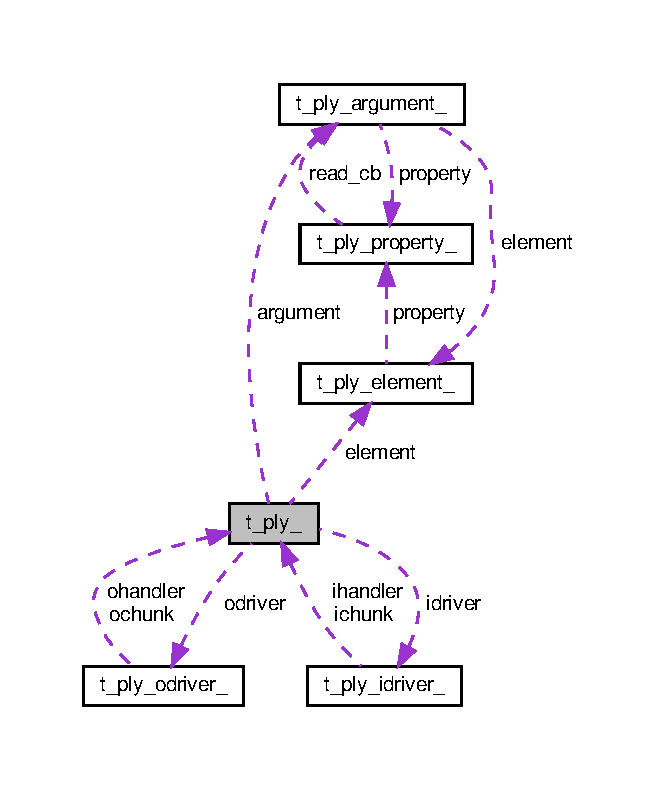
\includegraphics[width=316pt]{structt__ply____coll__graph}
\end{center}
\end{figure}
\subsection*{Public Attributes}
\begin{DoxyCompactItemize}
\item 
\mbox{\Hypertarget{structt__ply___a9be7c67e21b3920c3b7893d78f21c2e8}\label{structt__ply___a9be7c67e21b3920c3b7893d78f21c2e8}} 
e\+\_\+ply\+\_\+io\+\_\+mode {\bfseries io\+\_\+mode}
\item 
\mbox{\Hypertarget{structt__ply___a2feb88c586425471d4b6e786a4525207}\label{structt__ply___a2feb88c586425471d4b6e786a4525207}} 
e\+\_\+ply\+\_\+storage\+\_\+mode {\bfseries storage\+\_\+mode}
\item 
\mbox{\Hypertarget{structt__ply___a7de540782943375c56f31074be82d207}\label{structt__ply___a7de540782943375c56f31074be82d207}} 
\hyperlink{structt__ply__element__}{p\+\_\+ply\+\_\+element} {\bfseries element}
\item 
\mbox{\Hypertarget{structt__ply___a42fa31b10e98d40c726384903c4627c4}\label{structt__ply___a42fa31b10e98d40c726384903c4627c4}} 
long {\bfseries nelements}
\item 
\mbox{\Hypertarget{structt__ply___a3e3fe7d31c905da0fb259cdc9a99f47f}\label{structt__ply___a3e3fe7d31c905da0fb259cdc9a99f47f}} 
char $\ast$ {\bfseries comment}
\item 
\mbox{\Hypertarget{structt__ply___ab694821b90645fd2be0d8eb7c6d09fd2}\label{structt__ply___ab694821b90645fd2be0d8eb7c6d09fd2}} 
long {\bfseries ncomments}
\item 
\mbox{\Hypertarget{structt__ply___a515f90aa2fce385e0e7d235de8361b07}\label{structt__ply___a515f90aa2fce385e0e7d235de8361b07}} 
char $\ast$ {\bfseries obj\+\_\+info}
\item 
\mbox{\Hypertarget{structt__ply___abbc32008d7d5b85abd0d90ad3a701264}\label{structt__ply___abbc32008d7d5b85abd0d90ad3a701264}} 
long {\bfseries nobj\+\_\+infos}
\item 
\mbox{\Hypertarget{structt__ply___a0637e03cf8c826220eac2865e1c13cd4}\label{structt__ply___a0637e03cf8c826220eac2865e1c13cd4}} 
F\+I\+LE $\ast$ {\bfseries fp}
\item 
\mbox{\Hypertarget{structt__ply___ac390febe0010255e5d9439ab6f1d6fcd}\label{structt__ply___ac390febe0010255e5d9439ab6f1d6fcd}} 
int {\bfseries c}
\item 
\mbox{\Hypertarget{structt__ply___a6376859fab52fad26ba46db78c90a9bb}\label{structt__ply___a6376859fab52fad26ba46db78c90a9bb}} 
char {\bfseries buffer} \mbox{[}B\+U\+F\+F\+E\+R\+S\+I\+ZE\mbox{]}
\item 
\mbox{\Hypertarget{structt__ply___a09f60faf79c174f9ec79599a0b77e790}\label{structt__ply___a09f60faf79c174f9ec79599a0b77e790}} 
size\+\_\+t {\bfseries buffer\+\_\+first}
\item 
\mbox{\Hypertarget{structt__ply___a15e8ece9572100ce5213e8b221bf6057}\label{structt__ply___a15e8ece9572100ce5213e8b221bf6057}} 
size\+\_\+t {\bfseries buffer\+\_\+token}
\item 
\mbox{\Hypertarget{structt__ply___a1ae894dcae5850948a9855d9e449baec}\label{structt__ply___a1ae894dcae5850948a9855d9e449baec}} 
size\+\_\+t {\bfseries buffer\+\_\+last}
\item 
\mbox{\Hypertarget{structt__ply___aecaa80a70a03721553ebeab9fe9a22e0}\label{structt__ply___aecaa80a70a03721553ebeab9fe9a22e0}} 
\hyperlink{structt__ply__idriver__}{p\+\_\+ply\+\_\+idriver} {\bfseries idriver}
\item 
\mbox{\Hypertarget{structt__ply___ab76942a651062d0747637e8df5632e24}\label{structt__ply___ab76942a651062d0747637e8df5632e24}} 
\hyperlink{structt__ply__odriver__}{p\+\_\+ply\+\_\+odriver} {\bfseries odriver}
\item 
\mbox{\Hypertarget{structt__ply___affbe7e3e937f7f039f496d8a57b16904}\label{structt__ply___affbe7e3e937f7f039f496d8a57b16904}} 
\hyperlink{structt__ply__argument__}{t\+\_\+ply\+\_\+argument} {\bfseries argument}
\item 
\mbox{\Hypertarget{structt__ply___ad83687478a4c519a0840e6203cc92e81}\label{structt__ply___ad83687478a4c519a0840e6203cc92e81}} 
long {\bfseries welement}
\item 
\mbox{\Hypertarget{structt__ply___a3c1346b6f0538336dfa64b1db7c80545}\label{structt__ply___a3c1346b6f0538336dfa64b1db7c80545}} 
long {\bfseries wproperty}
\item 
\mbox{\Hypertarget{structt__ply___ad0eb60ffe6347b945be7773a4eb6b01c}\label{structt__ply___ad0eb60ffe6347b945be7773a4eb6b01c}} 
long {\bfseries winstance\+\_\+index}
\item 
\mbox{\Hypertarget{structt__ply___ad9286509435ac2873054e010dd3675e5}\label{structt__ply___ad9286509435ac2873054e010dd3675e5}} 
long {\bfseries wvalue\+\_\+index}
\item 
\mbox{\Hypertarget{structt__ply___ad8ac030b015c75d0cbb14cbb7f899b68}\label{structt__ply___ad8ac030b015c75d0cbb14cbb7f899b68}} 
long {\bfseries wlength}
\item 
\mbox{\Hypertarget{structt__ply___a3f9870cbe445137d16da2173363bc810}\label{structt__ply___a3f9870cbe445137d16da2173363bc810}} 
p\+\_\+ply\+\_\+error\+\_\+cb {\bfseries error\+\_\+cb}
\end{DoxyCompactItemize}


The documentation for this struct was generated from the following file\+:\begin{DoxyCompactItemize}
\item 
rply.\+c\end{DoxyCompactItemize}

\hypertarget{structt__ply__argument__}{}\section{t\+\_\+ply\+\_\+argument\+\_\+ Struct Reference}
\label{structt__ply__argument__}\index{t\+\_\+ply\+\_\+argument\+\_\+@{t\+\_\+ply\+\_\+argument\+\_\+}}


Collaboration diagram for t\+\_\+ply\+\_\+argument\+\_\+\+:\nopagebreak
\begin{figure}[H]
\begin{center}
\leavevmode
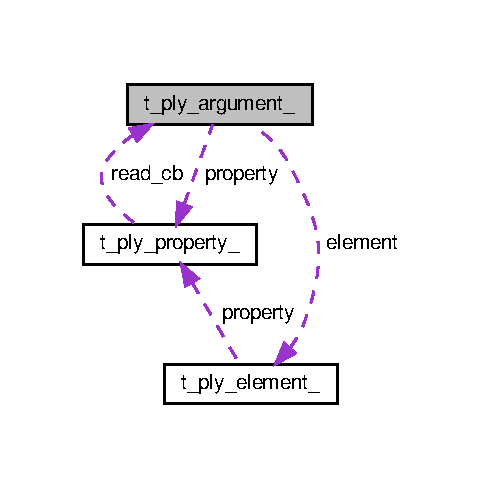
\includegraphics[width=232pt]{structt__ply__argument____coll__graph}
\end{center}
\end{figure}
\subsection*{Public Attributes}
\begin{DoxyCompactItemize}
\item 
\mbox{\Hypertarget{structt__ply__argument___a958bc37961f8ee44b39f72f0b221c0d7}\label{structt__ply__argument___a958bc37961f8ee44b39f72f0b221c0d7}} 
\hyperlink{structt__ply__element__}{p\+\_\+ply\+\_\+element} {\bfseries element}
\item 
\mbox{\Hypertarget{structt__ply__argument___ab0d8232410a2a77eb842892f3dddcb08}\label{structt__ply__argument___ab0d8232410a2a77eb842892f3dddcb08}} 
long {\bfseries instance\+\_\+index}
\item 
\mbox{\Hypertarget{structt__ply__argument___af38f3661a7ba2930c910027bd36790c4}\label{structt__ply__argument___af38f3661a7ba2930c910027bd36790c4}} 
\hyperlink{structt__ply__property__}{p\+\_\+ply\+\_\+property} {\bfseries property}
\item 
\mbox{\Hypertarget{structt__ply__argument___aaa7b3d7dca197835d72adaf12f9ec1ed}\label{structt__ply__argument___aaa7b3d7dca197835d72adaf12f9ec1ed}} 
long {\bfseries length}
\item 
\mbox{\Hypertarget{structt__ply__argument___a5b407c90440ee9f5a14b8816808cb658}\label{structt__ply__argument___a5b407c90440ee9f5a14b8816808cb658}} 
long {\bfseries value\+\_\+index}
\item 
\mbox{\Hypertarget{structt__ply__argument___ab4b092f2a002c13a39c251051d620b31}\label{structt__ply__argument___ab4b092f2a002c13a39c251051d620b31}} 
double {\bfseries value}
\item 
\mbox{\Hypertarget{structt__ply__argument___a33ffaef6d9affc8dd4322fff0856fd3e}\label{structt__ply__argument___a33ffaef6d9affc8dd4322fff0856fd3e}} 
void $\ast$ {\bfseries pdata}
\item 
\mbox{\Hypertarget{structt__ply__argument___a17560fa022ed7b8cffd9db501177a514}\label{structt__ply__argument___a17560fa022ed7b8cffd9db501177a514}} 
long {\bfseries idata}
\end{DoxyCompactItemize}


The documentation for this struct was generated from the following file\+:\begin{DoxyCompactItemize}
\item 
rply.\+c\end{DoxyCompactItemize}

\hypertarget{structt__ply__element__}{}\section{t\+\_\+ply\+\_\+element\+\_\+ Struct Reference}
\label{structt__ply__element__}\index{t\+\_\+ply\+\_\+element\+\_\+@{t\+\_\+ply\+\_\+element\+\_\+}}


Collaboration diagram for t\+\_\+ply\+\_\+element\+\_\+\+:\nopagebreak
\begin{figure}[H]
\begin{center}
\leavevmode
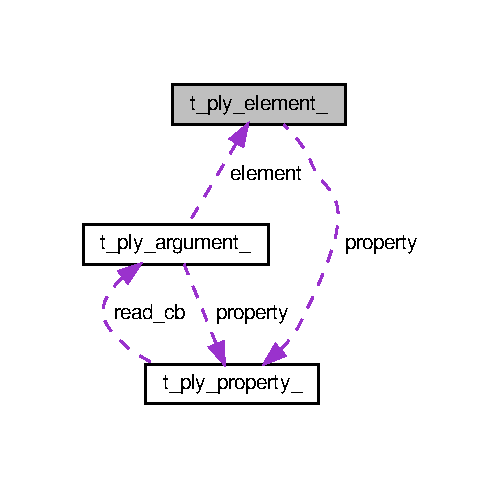
\includegraphics[width=242pt]{structt__ply__element____coll__graph}
\end{center}
\end{figure}
\subsection*{Public Attributes}
\begin{DoxyCompactItemize}
\item 
\mbox{\Hypertarget{structt__ply__element___a4190e367a648df18c038ef3cbe80e266}\label{structt__ply__element___a4190e367a648df18c038ef3cbe80e266}} 
char {\bfseries name} \mbox{[}W\+O\+R\+D\+S\+I\+ZE\mbox{]}
\item 
\mbox{\Hypertarget{structt__ply__element___a742314a40fcbc69660907d9be9ae4927}\label{structt__ply__element___a742314a40fcbc69660907d9be9ae4927}} 
long {\bfseries ninstances}
\item 
\mbox{\Hypertarget{structt__ply__element___adf2e07d9d09ac4c1152c396f88bf8ddc}\label{structt__ply__element___adf2e07d9d09ac4c1152c396f88bf8ddc}} 
\hyperlink{structt__ply__property__}{p\+\_\+ply\+\_\+property} {\bfseries property}
\item 
\mbox{\Hypertarget{structt__ply__element___a604596912c74d0521a02561884c1ffa9}\label{structt__ply__element___a604596912c74d0521a02561884c1ffa9}} 
long {\bfseries nproperties}
\end{DoxyCompactItemize}


The documentation for this struct was generated from the following file\+:\begin{DoxyCompactItemize}
\item 
rply.\+c\end{DoxyCompactItemize}

\hypertarget{structt__ply__idriver__}{}\section{t\+\_\+ply\+\_\+idriver\+\_\+ Struct Reference}
\label{structt__ply__idriver__}\index{t\+\_\+ply\+\_\+idriver\+\_\+@{t\+\_\+ply\+\_\+idriver\+\_\+}}


Collaboration diagram for t\+\_\+ply\+\_\+idriver\+\_\+\+:\nopagebreak
\begin{figure}[H]
\begin{center}
\leavevmode
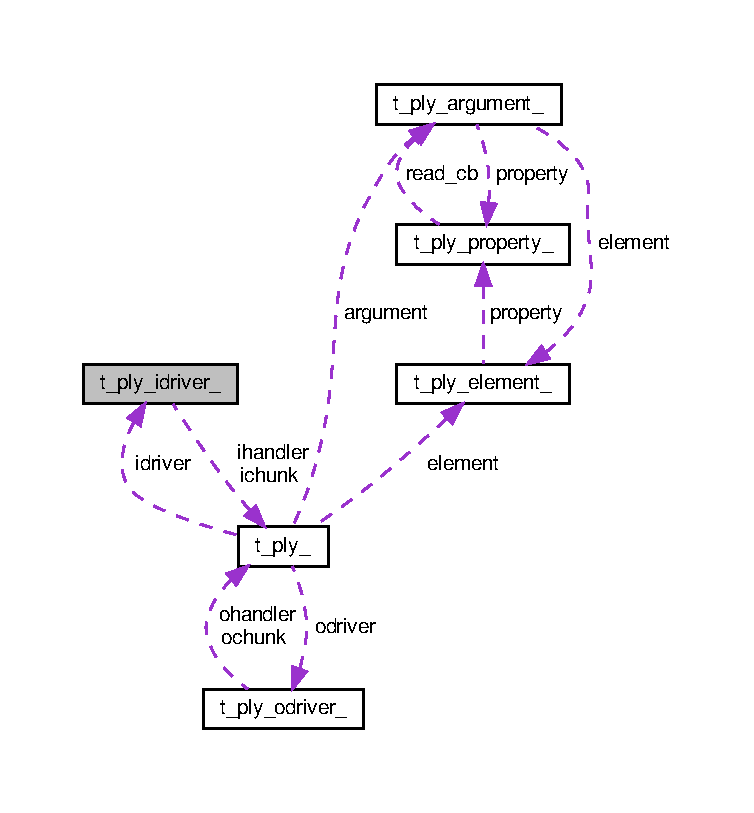
\includegraphics[width=350pt]{structt__ply__idriver____coll__graph}
\end{center}
\end{figure}
\subsection*{Public Attributes}
\begin{DoxyCompactItemize}
\item 
\mbox{\Hypertarget{structt__ply__idriver___afabd4f3eef6f708d9872c623f5d48324}\label{structt__ply__idriver___afabd4f3eef6f708d9872c623f5d48324}} 
p\+\_\+ply\+\_\+ihandler {\bfseries ihandler} \mbox{[}16\mbox{]}
\item 
\mbox{\Hypertarget{structt__ply__idriver___a317e387dd6c97231d081c71b5e705b28}\label{structt__ply__idriver___a317e387dd6c97231d081c71b5e705b28}} 
p\+\_\+ply\+\_\+ichunk {\bfseries ichunk}
\item 
\mbox{\Hypertarget{structt__ply__idriver___a51009fbc3df6433214fd19a34f0aac02}\label{structt__ply__idriver___a51009fbc3df6433214fd19a34f0aac02}} 
const char $\ast$ {\bfseries name}
\end{DoxyCompactItemize}


The documentation for this struct was generated from the following file\+:\begin{DoxyCompactItemize}
\item 
rply.\+c\end{DoxyCompactItemize}

\hypertarget{structt__ply__odriver__}{}\section{t\+\_\+ply\+\_\+odriver\+\_\+ Struct Reference}
\label{structt__ply__odriver__}\index{t\+\_\+ply\+\_\+odriver\+\_\+@{t\+\_\+ply\+\_\+odriver\+\_\+}}


Collaboration diagram for t\+\_\+ply\+\_\+odriver\+\_\+\+:\nopagebreak
\begin{figure}[H]
\begin{center}
\leavevmode
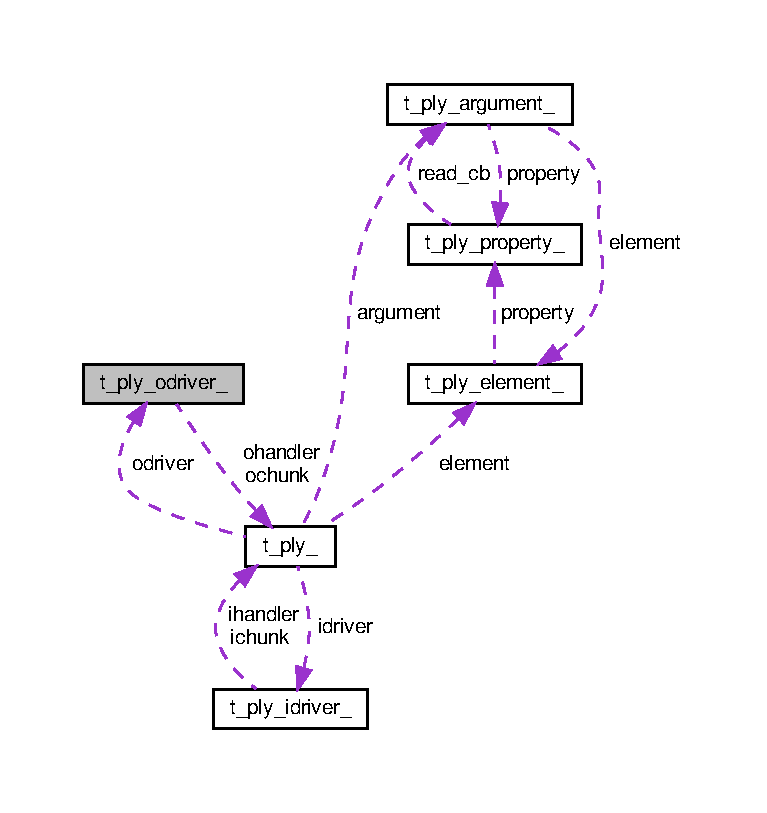
\includegraphics[width=350pt]{structt__ply__odriver____coll__graph}
\end{center}
\end{figure}
\subsection*{Public Attributes}
\begin{DoxyCompactItemize}
\item 
\mbox{\Hypertarget{structt__ply__odriver___a8e73dd635a21a1be2de07c7ead55fb44}\label{structt__ply__odriver___a8e73dd635a21a1be2de07c7ead55fb44}} 
p\+\_\+ply\+\_\+ohandler {\bfseries ohandler} \mbox{[}16\mbox{]}
\item 
\mbox{\Hypertarget{structt__ply__odriver___a02635ba242394795d3716793cd1c3c87}\label{structt__ply__odriver___a02635ba242394795d3716793cd1c3c87}} 
p\+\_\+ply\+\_\+ochunk {\bfseries ochunk}
\item 
\mbox{\Hypertarget{structt__ply__odriver___a510d75a4c2aa06c9266de2554636f600}\label{structt__ply__odriver___a510d75a4c2aa06c9266de2554636f600}} 
const char $\ast$ {\bfseries name}
\end{DoxyCompactItemize}


The documentation for this struct was generated from the following file\+:\begin{DoxyCompactItemize}
\item 
rply.\+c\end{DoxyCompactItemize}

\hypertarget{structt__ply__property__}{}\section{t\+\_\+ply\+\_\+property\+\_\+ Struct Reference}
\label{structt__ply__property__}\index{t\+\_\+ply\+\_\+property\+\_\+@{t\+\_\+ply\+\_\+property\+\_\+}}


Collaboration diagram for t\+\_\+ply\+\_\+property\+\_\+\+:\nopagebreak
\begin{figure}[H]
\begin{center}
\leavevmode
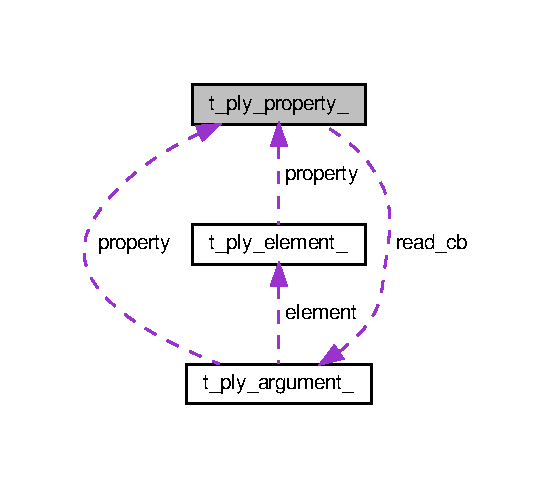
\includegraphics[width=265pt]{structt__ply__property____coll__graph}
\end{center}
\end{figure}
\subsection*{Public Attributes}
\begin{DoxyCompactItemize}
\item 
\mbox{\Hypertarget{structt__ply__property___a9093045e79e9eafa04d290b7bdc2e83b}\label{structt__ply__property___a9093045e79e9eafa04d290b7bdc2e83b}} 
char {\bfseries name} \mbox{[}W\+O\+R\+D\+S\+I\+ZE\mbox{]}
\item 
\mbox{\Hypertarget{structt__ply__property___a7021be56bf6726be847887cfbba0d24e}\label{structt__ply__property___a7021be56bf6726be847887cfbba0d24e}} 
e\+\_\+ply\+\_\+type {\bfseries type}
\item 
\mbox{\Hypertarget{structt__ply__property___a3caa07217f713492cf06016c7654e87f}\label{structt__ply__property___a3caa07217f713492cf06016c7654e87f}} 
e\+\_\+ply\+\_\+type {\bfseries value\+\_\+type}
\item 
\mbox{\Hypertarget{structt__ply__property___af9b3b45ae24c1fd7d9d81a18bc3f76a7}\label{structt__ply__property___af9b3b45ae24c1fd7d9d81a18bc3f76a7}} 
e\+\_\+ply\+\_\+type {\bfseries length\+\_\+type}
\item 
\mbox{\Hypertarget{structt__ply__property___af139cc44e475f4754daf7501e1288716}\label{structt__ply__property___af139cc44e475f4754daf7501e1288716}} 
p\+\_\+ply\+\_\+read\+\_\+cb {\bfseries read\+\_\+cb}
\item 
\mbox{\Hypertarget{structt__ply__property___af53fa1cccd547dddd25d2ea111fd3159}\label{structt__ply__property___af53fa1cccd547dddd25d2ea111fd3159}} 
void $\ast$ {\bfseries pdata}
\item 
\mbox{\Hypertarget{structt__ply__property___a87447519f61802d3c7a4fef1024c1d03}\label{structt__ply__property___a87447519f61802d3c7a4fef1024c1d03}} 
long {\bfseries idata}
\end{DoxyCompactItemize}


The documentation for this struct was generated from the following file\+:\begin{DoxyCompactItemize}
\item 
rply.\+c\end{DoxyCompactItemize}

\chapter{File Documentation}
\hypertarget{icp_8h}{}\section{icp.\+h File Reference}
\label{icp_8h}\index{icp.\+h@{icp.\+h}}


S\+C\+A\+LE I\+CP adjusted class.  


{\ttfamily \#include $<$iostream$>$}\newline
{\ttfamily \#include $<$fstream$>$}\newline
{\ttfamily \#include $<$cstdio$>$}\newline
{\ttfamily \#include $<$pcl/io/ply\+\_\+io.\+h$>$}\newline
{\ttfamily \#include $<$pcl/point\+\_\+cloud.\+h$>$}\newline
{\ttfamily \#include $<$pcl/surface/gp3.\+h$>$}\newline
{\ttfamily \#include $<$opencv2/core/core.\+hpp$>$}\newline
{\ttfamily \#include $<$opencv2/highgui/highgui.\+hpp$>$}\newline
{\ttfamily \#include \char`\"{}Matlab\+Data\+Array.\+hpp\char`\"{}}\newline
{\ttfamily \#include \char`\"{}Matlab\+Engine.\+hpp\char`\"{}}\newline
{\ttfamily \#include \char`\"{}rply.\+h\char`\"{}}\newline
Include dependency graph for icp.\+h\+:\nopagebreak
\begin{figure}[H]
\begin{center}
\leavevmode
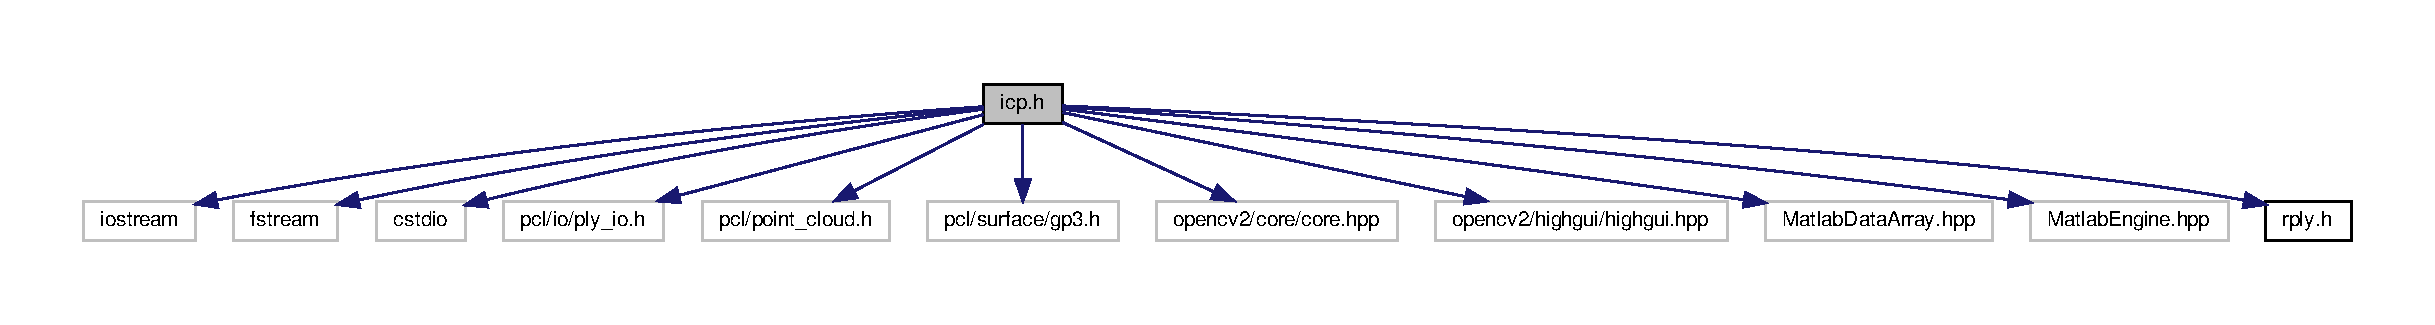
\includegraphics[width=350pt]{icp_8h__incl}
\end{center}
\end{figure}
\subsection*{Classes}
\begin{DoxyCompactItemize}
\item 
class \hyperlink{classaPoint}{a\+Point}
\begin{DoxyCompactList}\small\item\em Class to handle points. \end{DoxyCompactList}\item 
class \hyperlink{classPoints3D}{Points3D}
\begin{DoxyCompactList}\small\item\em Class to handle 3D points. \end{DoxyCompactList}\item 
class \hyperlink{classPoints3Dvec}{Points3\+Dvec}
\begin{DoxyCompactList}\small\item\em Class to handle Point vectors. \end{DoxyCompactList}\item 
class \hyperlink{classicp}{icp}
\begin{DoxyCompactList}\small\item\em Main I\+CP class. \end{DoxyCompactList}\end{DoxyCompactItemize}


\subsection{Detailed Description}
S\+C\+A\+LE I\+CP adjusted class. 

\begin{DoxyAuthor}{Author}
Esteban Andrade 
\end{DoxyAuthor}
\begin{DoxyVersion}{Version}
0.\+1 
\end{DoxyVersion}
\begin{DoxyDate}{Date}
2021-\/06-\/07
\end{DoxyDate}
\begin{DoxyCopyright}{Copyright}
Copyright (c) 2021 
\end{DoxyCopyright}

\hypertarget{Reconstruction_8h}{}\section{Reconstruction.\+h File Reference}
\label{Reconstruction_8h}\index{Reconstruction.\+h@{Reconstruction.\+h}}


This is the main class be used to hold all the A\+PI used for data processing.  


{\ttfamily \#include $<$pcl/common/common\+\_\+headers.\+h$>$}\newline
{\ttfamily \#include $<$pcl/features/normal\+\_\+3d.\+h$>$}\newline
{\ttfamily \#include $<$pcl/console/parse.\+h$>$}\newline
{\ttfamily \#include $<$pcl/common/common.\+h$>$}\newline
{\ttfamily \#include $<$pcl/io/obj\+\_\+io.\+h$>$}\newline
{\ttfamily \#include $<$pcl/filters/statistical\+\_\+outlier\+\_\+removal.\+h$>$}\newline
{\ttfamily \#include $<$pcl/kdtree/kdtree\+\_\+flann.\+h$>$}\newline
{\ttfamily \#include $<$pcl/kdtree/kdtree.\+h$>$}\newline
{\ttfamily \#include $<$pcl/kdtree/flann.\+h$>$}\newline
{\ttfamily \#include $<$pcl/kdtree/impl/io.\+hpp$>$}\newline
{\ttfamily \#include $<$pcl/kdtree/impl/kdtree\+\_\+flann.\+hpp$>$}\newline
{\ttfamily \#include $<$pcl/surface/mls.\+h$>$}\newline
{\ttfamily \#include $<$pcl/features/integral\+\_\+image\+\_\+normal.\+h$>$}\newline
{\ttfamily \#include $<$pcl/sample\+\_\+consensus/method\+\_\+types.\+h$>$}\newline
{\ttfamily \#include $<$pcl/sample\+\_\+consensus/model\+\_\+types.\+h$>$}\newline
{\ttfamily \#include $<$pcl/segmentation/sac\+\_\+segmentation.\+h$>$}\newline
{\ttfamily \#include $<$pcl/\+Model\+Coefficients.\+h$>$}\newline
{\ttfamily \#include $<$pcl/io/pcd\+\_\+io.\+h$>$}\newline
{\ttfamily \#include $<$pcl/point\+\_\+types.\+h$>$}\newline
{\ttfamily \#include $<$pcl/filters/extract\+\_\+indices.\+h$>$}\newline
{\ttfamily \#include $<$pcl/filters/passthrough.\+h$>$}\newline
{\ttfamily \#include $<$pcl/segmentation/extract\+\_\+clusters.\+h$>$}\newline
{\ttfamily \#include $<$pcl/surface/poisson.\+h$>$}\newline
{\ttfamily \#include $<$pcl/io/ply\+\_\+io.\+h$>$}\newline
{\ttfamily \#include $<$pcl/io/io.\+h$>$}\newline
{\ttfamily \#include $<$pcl/io/vtk\+\_\+lib\+\_\+io.\+h$>$}\newline
{\ttfamily \#include $<$pcl/point\+\_\+cloud.\+h$>$}\newline
{\ttfamily \#include $<$pcl/\+Polygon\+Mesh.\+h$>$}\newline
{\ttfamily \#include $<$pcl/\+Texture\+Mesh.\+h$>$}\newline
{\ttfamily \#include $<$pcl/pcl\+\_\+macros.\+h$>$}\newline
{\ttfamily \#include $<$pcl/conversions.\+h$>$}\newline
{\ttfamily \#include $<$pcl/range\+\_\+image/range\+\_\+image\+\_\+planar.\+h$>$}\newline
{\ttfamily \#include $<$pcl/io/impl/vtk\+\_\+lib\+\_\+io.\+hpp$>$}\newline
{\ttfamily \#include $<$iostream$>$}\newline
{\ttfamily \#include $<$thread$>$}\newline
{\ttfamily \#include $<$chrono$>$}\newline
{\ttfamily \#include $<$string$>$}\newline
{\ttfamily \#include $<$algorithm$>$}\newline
{\ttfamily \#include $<$boost/filesystem.\+hpp$>$}\newline
{\ttfamily \#include $<$ctime$>$}\newline
{\ttfamily \#include $<$boost/thread/thread.\+hpp$>$}\newline
{\ttfamily \#include $<$flann/flann.\+hpp$>$}\newline
{\ttfamily \#include $<$pcl/common/pca.\+h$>$}\newline
{\ttfamily \#include $<$pcl/filters/voxel\+\_\+grid.\+h$>$}\newline
{\ttfamily \#include $<$unsupported/\+Eigen/\+Matrix\+Functions$>$}\newline
Include dependency graph for Reconstruction.\+h\+:\nopagebreak
\begin{figure}[H]
\begin{center}
\leavevmode

\includegraphics[width=350pt]{Reconstruction_8h__incl}
\end{center}
\end{figure}
\subsection*{Classes}
\begin{DoxyCompactItemize}
\item 
class \hyperlink{classReconstruction}{Reconstruction}
\begin{DoxyCompactList}\small\item\em The Class \hyperlink{classReconstruction}{Reconstruction} is used process the target pointcloud. It contain many implemeted algorithms used for filtering, segmentation, clusteting, etc. \end{DoxyCompactList}\end{DoxyCompactItemize}


\subsection{Detailed Description}
This is the main class be used to hold all the A\+PI used for data processing. 

\begin{DoxyAuthor}{Author}
Esteban Andrade 
\end{DoxyAuthor}
\begin{DoxyVersion}{Version}
0.\+1 
\end{DoxyVersion}
\begin{DoxyDate}{Date}
2021-\/06-\/07
\end{DoxyDate}
\begin{DoxyCopyright}{Copyright}
Copyright (c) 2021 
\end{DoxyCopyright}

%--- End generated contents ---

% Index
\backmatter
\newpage
\phantomsection
\clearemptydoublepage
\addcontentsline{toc}{chapter}{Index}
\printindex

\end{document}
